%%% Building a Zinc+-style F2Z prover for SHA-256 -------------------------
%%
%%  Build:  latexmk -pdf main.tex
%%
%%  Audience: ZK engineers fluent in sumcheck and passingly familiar with FRI.
%%  Assumes no prior exposure to F2Z, Zinc+, PIMSAT or ring-switching.
%%
%%  Sources of truth:
%%    paper/main.tex            F2Z (Overleaf-synced, branch master)
%%    ~/Downloads/zinc+.pdf     Zinc+, Section 8.2 = the SHA-256 arithmetization
%%    src/taps.rs               the lane-crossing virtualization
%%    src/pcs.rs                exponent fold, bit layout, GF(2^128)
%%    src/ligerito_flock.rs     commit path, ring-switch, recursive Ligerito
%%    docs/blake3-taps-design.md  the cost-model-driven arithmetization method
%%
%% -------------------------------------------------------------------------
\documentclass[11pt,letterpaper]{article}

%% Wide outer margin: the claim ledger lives there, ~1/5 of the page.
\usepackage[letterpaper,
            left=0.85in, right=0.45in, top=0.95in, bottom=1.0in,
            marginparwidth=1.72in, marginparsep=0.13in, includemp]{geometry}

\usepackage{amsmath,amssymb,amsthm}
\allowdisplaybreaks
\usepackage{booktabs}
\usepackage{array}
\usepackage{longtable}
\usepackage{enumitem}
\usepackage{microtype}
\usepackage{xcolor}
\usepackage{float}
\usepackage{tikz}
\usetikzlibrary{positioning, arrows.meta, calc, decorations.pathreplacing, fit}
\usepackage{caption}
\usepackage[colorlinks=true,
            linkcolor=blue!50!black,
            citecolor=blue!50!black,
            urlcolor=blue!50!black]{hyperref}
\usepackage[capitalize,nameinlink]{cleveref}

\usepackage[T1]{fontenc}
\usepackage{lmodern}
\usepackage{anyfontsize}
\usepackage{shanotation}
\usepackage{claimledger}

\tolerance=1600
\setlength{\emergencystretch}{1.8em}
\hbadness=2500

\theoremstyle{definition}
\newtheorem{definition}{Definition}[section]
\newtheorem{remark}[definition]{Remark}
\newtheorem{example}[definition]{Example}
\newtheorem{warning}[definition]{Warning}
\theoremstyle{plain}
\newtheorem{lemma}[definition]{Lemma}

\crefname{definition}{Definition}{Definitions}
\crefname{remark}{Remark}{Remarks}
\crefname{warning}{Warning}{Warnings}
\Crefname{warning}{Warning}{Warnings}
%% `step' environments \refstepcounter{clgstep}; teach cleveref to name them.
\crefname{clgstep}{Step}{Steps}
\Crefname{clgstep}{Step}{Steps}

\title{\textbf{Proving SHA-256 with F2Z}\\[3pt]
  \large A Zinc\raisebox{0.1ex}{+}-style construction, end to end:\\
  arithmetization, commitment, zero-check, opening}
\author{The \code{f2z-pcs} repository}
\date{\today}

\begin{document}
\maketitle

\begin{abstract}
\noindent
This note builds a SHA-256 prover on F2Z from the ground up. The design has one
governing idea: \emph{commit bits, derive everything else}. A public
$\Ftwo$-matrix $M$ manufactures every XOR SHA-256 needs as a \emph{virtual}
witness $\hh$ that is never committed; rotations and shifts fall out for free as
permuted power-of-two diagonals in the constraint matrix. What is left is purely
$\Z$-linear --- no quadratic terms, no lookups, no ideals, and no second ring.

The consequences are worth stating up front, because they are what makes the
construction worth learning. Ten Zinc\raisebox{0.1ex}{+} constraint families
collapse to three. All ten bit-ness lookups and all three
$\Ch$/$\Maj$ lookups disappear. So does the $\Ftwo[X]$ trace component, and so
do the ideals --- with a bit witness there is no module, no degree bound, and
none of the padding risk that a shared $(d,B)$ typing carries.
And because every constraint is linear, the nonlinear outer sumcheck vanishes
outright --- there is no Hadamard product for it to handle.  The inner
evaluation-shaping sumcheck does \emph{not} vanish.  Collapsing the public
matrix produces a general coefficient vector
$\vv=\bar A^{\!\top}\eq(\cdot,r_{\rm con})$, whereas the tensorized F2Z opening
needs weights that separate across its row and column axes.  A degree-$2$
sumcheck therefore reduces the general claim to one with weights
$c\,\eq(\cdot,r_h)$ before any coefficient is lifted to $\Z$.  This is the
load-bearing interface between the PIOP and F2Z, not an optional optimization.
The verifier still performs the public sparse collapse; its circuit-dependent
part is $N$-free by uniformity, while reading $N$ independent public inputs is
still $\Theta(N)$.  Existing repository timings primarily measure the opening
after this PIOP, so the new $\Theta(|\hh|)$ field pass must be included before
quoting an end-to-end prover percentage.

We assume fluency with sumcheck and passing familiarity with FRI-style
proximity testing. We assume nothing about F2Z, Zinc\raisebox{0.1ex}{+},
PIMSAT, or ring-switching.

\Cref{sec:arith} builds the arithmetization. \Cref{sec:commit} commits the
witness, with diagrams. \Cref{sec:piop,sec:iopp} walk the two protocol halves,
each carrying a margin ledger of the claims still open --- colour-coded so that
reading only the margin shows the statement being dismantled.  The PIOP has
four steps and ends at the separable claim
$E_{\rm eq}:\ipq{c\,\eq(\cdot,r_h)}{\pi_q(\hh)}=\tau$.  The opening IOP then
has seven steps: integer column folds, the exponent fold, merged GKR, the
row-only pre-sumcheck, full virtualization elimination, ring-switching, and the
proximity opening.  One standing claim, $H$: ``$\hh$ really is $M$ applied to
$\ff^{\circ}$'', survives the whole PIOP and is discharged by the full
transpose in \cref{sec:iopp}. That claim is the spine of the document.
\end{abstract}

\setcounter{tocdepth}{2}
{\parskip=0pt\tableofcontents}

\clearpage
\section{Arithmetizing SHA-256}\label{sec:arith}

\subsection{The idea in one page}

SHA-256 does two kinds of work, and they want opposite things from a proof
system.

\begin{center}\small
\begin{tabular}{@{}lll@{}}
\toprule
& operations & wants \\
\midrule
\textbf{bit shuffling} & $\ROTR^r$, $\SHR^r$, $\xo$ & characteristic 2, where
  XOR is addition\\
\textbf{arithmetic} & $+ \bmod 2^{32}$ & the integers, where carries mean
  something\\
\bottomrule
\end{tabular}
\end{center}

Systems that pick one pay for the other. Arithmetize over $\Fq$ and every XOR
becomes a pile of range-checked limbs; arithmetize over $\Ftwo$ and every
addition becomes a ripple-carry circuit.

F2Z does neither, because its commitment holds \emph{bits}, and bits are the one
thing both characteristics agree on. Two moves follow, and between them they
account for the whole arithmetization:

\begin{quote}
\textbf{(i) Every $\Ftwo$-linear function of the committed bits is free.} Do not
constrain it and do not commit it --- \emph{derive} it with a public
$\Ftwo$-matrix $M$, and let the verifier absorb $M$ into its own coefficients at
the very end of the protocol.

\textbf{(ii) Words are assembled inside the constraint system.} A $32$-bit value
is $\sum_i b_i 2^i$ --- a $\Z$-linear form on committed bits. Word assembly is a
row of $A$, not a separate object.
\end{quote}

Move (ii) has a consequence worth stating loudly, because it removes an entire
layer that earlier drafts of this construction carried: \textbf{permute that
diagonal and rotations and shifts come for free.}
\[
  \ROTR^r(a) \;=\; \sum_{i=0}^{31} a_{(i+r)\bmod 32}\,2^i ,
  \qquad
  \SHR^r(a) \;=\; \sum_{i=0}^{31-r} a_{i+r}\,2^i .
\]
Both are $\Z$-linear forms on the \emph{same} committed bits --- zero rows in
$M$, zero slots in $\hh$, zero commitment. So $M$ never has to express a
rotation, and the only thing it does is XOR.

What is left is one linear system over $\Z$: no ideals, no polynomial ring, no
quadratic terms, no lookups.

\begin{center}
\begin{tikzpicture}[
  font=\scriptsize,
  bx/.style={draw=black!45, rounded corners=1.6pt, align=center,
             inner sep=3.5pt, line width=0.4pt, minimum height=0.6cm},
  f2/.style={bx, fill=blue!9},
  zz/.style={bx, fill=orange!13},
  ar/.style={-{Latex[length=1.7mm]}, draw=black!55, line width=0.5pt},
  lb/.style={font=\tiny, text=black!55, align=center},
]
\node[bx, fill=black!6] (f) at (0,0) {$\ff\in\bits^{\ell}$\\committed bits};
\node[f2] (m) at (3.15,0.80) {$M \in \Ftwo^{|\hh|\times|\ff|}$\\\textbf{XOR only}};
\node[f2] (h) at (6.35,0.80) {$\hh$\\virtual, not committed};
\node[zz] (a) at (6.35,-0.90) {$A$ over $\Z$\\word assembly $+$ adds};
\node[bx, fill=green!10] (o) at (9.5,0) {$A_{\xx}^{\circ}\hh^{\circ}=0$ over $\Z$};

\draw[ar] (f) -- (m); \draw[ar] (m) -- (h);
\draw[ar] (f) |- (a);
\draw[ar] (h) -| (9.5,0.44); \draw[ar] (a) -| (9.5,-0.44);
\node[lb, text=blue!45!black] at (4.75,1.48) {characteristic 2 --- free};
\node[lb, text=orange!55!black] at (4.30,-1.42) {characteristic $q$ --- the only constraints};
\end{tikzpicture}
\captionof{figure}{The split. $M$ manufactures every XOR; after public data are
substituted into $A_{\xx}^{\circ}$, $A$ assembles words
(rotations free, by permuting the power-of-two diagonal) and states the modular
additions. One linear system, one ring.}\label{fig:split}
\end{center}

\begin{remark}[Why there are no ideals here]\label{rem:noideals}
Earlier versions of this construction carried the witness in $\Z^{\leq31}_{\leq
B}[X]$ and stated the modular additions as membership in the ideal $(X-2)$,
where $p\in(X-2)\iff p(2)=0$. That machinery is the paper's general
\textsc{PIMSAT} construction, and for hashes it buys nothing --- evaluating
membership at $X=2$ gives
\[
  \hat y - \textstyle\sum_j \hat x_j + \mu X^{32} \in (X-2)
  \qquad\Longleftrightarrow\qquad
  y - \textstyle\sum_j x_j + \mu\,2^{32} = 0 \ \text{ over } \Z,
\]
which is the row we write anyway. Same equation, unused indeterminate. Dropping
it removes a prover message, a full prover pass, and --- most importantly --- the
typing problem of \cref{rem:typing}.

Ideals are not vestigial in general. They earn their place for lattice
relations, where a computation in $R[X]/I$ genuinely does not care which
representative appears, so $c-ab\in I$ suffices; without them you would either
commit the quotient or let $c$'s degree grow, and both cost committed bits.
Hashes are the opposite case --- a register value must be a minimal
representative immediately, so the ideal does not discharge the obligation.
\end{remark}

\begin{remark}[Only monic generators are available anyway]
Even if you wanted the ideal, the one you would reach for is unavailable. The
projection $\pi_q$ must send $I$ to a \emph{proper} ideal of $\Fq[X]$; if $I$
contains an integer coprime to $q$ its image contains a unit and the membership
check becomes vacuous. So $(2^{32})$ --- the natural way to say ``equal modulo
$2^{32}$'' --- is excluded, and only monic generators survive. That is why the
ideal route has to express the modulus as the place-value term $\mu X^{32}$
under $(X-2)$ rather than saying it directly.
\end{remark}

\subsection{Two ways to type the witness}\label{sec:typing}

The choice made above --- a bit witness rather than a polynomial one --- is the
one decision that shapes everything after it, and it is easy to mis-frame as a
dichotomy when it is not.

\paragraph{The committed data is the same either way.}
A bit-polynomial $\hat w(X)=\sum_{i<32}w_iX^i$ with $w_i\in\bits$ \emph{is}
thirty-two bits. The $[X]$ is a label saying ``these thirty-two belong
together''; nothing extra is stored, and the commitment of \cref{sec:commit}
packs the identical bit stream in both cases. So the question is never
``polynomials or bits''. It is:

\begin{quote}
\textbf{Who owns the grouping of bits into words --- the witness type, or the
constraint matrix?}
\end{quote}

\begin{center}
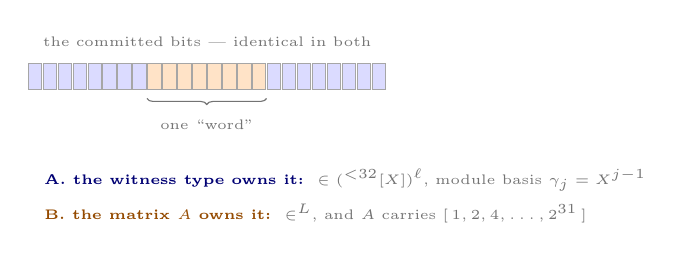
\begin{tikzpicture}[
  font=\scriptsize,
  bitc/.style={draw=black!35, minimum width=0.17cm, minimum height=0.34cm,
              inner sep=0pt, line width=0.25pt},
  hlA/.style={fill=blue!14}, hlB/.style={fill=orange!22},
  dcap/.style={font=\tiny, text=black!55, align=center},
  lbl/.style={font=\scriptsize\bfseries},
]
\foreach \k in {0,...,23} {
  \pgfmathsetmacro\bx{\k*0.19}
  \ifnum\k<8 \node[bitc, hlA] at (\bx,0) {}; \else
    \ifnum\k<16 \node[bitc, hlB] at (\bx,0) {}; \else
      \node[bitc, hlA] at (\bx,0) {}; \fi\fi
}
\node[dcap] at (2.19,0.44) {the committed bits --- identical in both};
\draw[decorate, decoration={brace, amplitude=2.2pt, mirror}, draw=black!55]
  (8*0.19-0.095,-0.28) -- (15*0.19+0.095,-0.28);
\node[dcap] at (2.19,-0.62) {one ``word''};

%% A and B stacked BELOW the strip: placed beside it they overlapped its right end.
\node[dcap, anchor=west, align=left] at (0,-1.32)
  {\textbf{\textcolor{blue!45!black}{A. the witness type owns it:}}\ \
   $\ff\in(\bits^{<32}[X])^{\ell}$, module basis $\gamma_j=X^{j-1}$};
\node[dcap, anchor=west, align=left] at (0,-1.74)
  {\textbf{\textcolor{orange!58!black}{B. the matrix $A$ owns it:}}\ \
   $\ff\in\bits^{L}$, and $A$ carries $[\,1,2,4,\dots,2^{31}\,]$};
\end{tikzpicture}
\end{center}

\begin{center}\small
\begin{tabular}{@{}p{0.14\textwidth}p{0.22\textwidth}p{0.23\textwidth}@{}}
\toprule
& \textbf{A. polynomial witness} & \textbf{B. bit witness}\\
\midrule
witness type & $(\Z^{\leq31}_{\leq B}[X])^{\ell}$ & $\bits^{L}$\\
$(d,B)$ & $d=31$, $B$ per column & $d=0$, $B=1$\\
grouping lives in & the module basis & $A$'s coefficients\\
$M$ outputs & words & bits\\
rotations, shifts & need $M$ --- a word-level $\ROTR$ is not $\Z$-linear
  & \textbf{free} --- a permuted coefficient pattern\\
modular addition & ideal $(X-2)$, carry monomial $X^{32}$ & plain $\Z$ row,
  carry term $2^{32}\mu$\\
ideals & required & none\\
opening carries & $\psi_M(\gamma_j)=\alpha^{j-1}$ in the coefficient vector
  & nothing extra\\
typing risk & shared $(d,B)$ pads $3$-bit carries to $32$ & none --- every cell
  is one bit\\
\bottomrule
\end{tabular}
\end{center}

The row that decides it for hashes is the fourth. Under A a rotation of a
\emph{word} is not a $\Z$-linear function of that word, so $M$ must manufacture
it and the result occupies a slot in $\hh$. Under B the word is already
$\sum_i b_i2^i$, so the rotation is the same coefficient pattern permuted --- and
costs nothing anywhere. That is what leaves $M$ responsible for XOR alone.

\paragraph{When the polynomial witness is the right choice.}
A is not a worse design; it is a design for a different workload. Where the
computation is \emph{natively} over a polynomial ring --- lattice signatures such
as Falcon, or anything in $R[X]/I$ --- the ideal earns its place, for the reason
in \cref{rem:noideals}: a product can be constrained as $c-ab\in I$ without
pinning down which representative of $c \bmod I$ the prover used. There is a
protocol-level argument too: ideal membership with the zero ideal degenerates to
univariate skip, so the general form is a \emph{generalised} univariate skip
rather than mere notation.

Hashes are the opposite case, and the reason is the next round: a register value
is immediately consumed bit-by-bit, so it must already be a minimal
representative and $c-ab\in I$ does not discharge the obligation.

\begin{remark}[One relation, two instantiations]\label{rem:oneinstance}
A and B are not competing systems. B is the degenerate case of the same
\textsc{PIMSAT} relation at $d=0$, $B=1$: the module collapses to $\Z$, $[X]$
goes unused, and the ideal becomes $(0)$. Nothing below the arithmetization
changes --- the commitment path of \cref{sec:commit}, the exponent fold, GKR, the
ring-switch and the proximity test are identical. Only the top layer differs.
\end{remark}

\subsection{All of SHA-256, in one table}\label{sec:shaspec}

SHA-256's compression function keeps eight $32$-bit registers $a,\dots,h$, runs
$64$ rounds, and first expands a $16$-word message block into a $64$-word
schedule. That is the whole of it --- and the whole of it fits in
\cref{tab:sha}.

Read the table with one convention: \textbf{every quantity is a $32$-bit word},
$+$ means addition modulo $2^{32}$, and $\xo$, $\wedge$, $\neg$ are bitwise XOR,
AND and NOT. $\ROTR^r$ rotates right by $r$; $\SHR^r$ shifts right by $r$ and
fills with zeros. Nothing else is needed.

\begin{center}\small
\begin{tabular}{@{}>{\raggedright\arraybackslash}p{0.13\textwidth}
                  >{\raggedright\arraybackslash}p{0.34\textwidth}
                  >{\raggedright\arraybackslash}p{0.21\textwidth}@{}}
\toprule
quantity & definition & where it goes\\
\midrule
\multicolumn{3}{@{}l}{\emph{Bit-mixing functions}}\\
$\Sigma_0(x)$ & $\ROTR^{2}(x)\xo\ROTR^{13}(x)\xo\ROTR^{22}(x)$
  & rotations free in $A$; XOR in $M$\\
$\Sigma_1(x)$ & $\ROTR^{6}(x)\xo\ROTR^{11}(x)\xo\ROTR^{25}(x)$ & same\\
$\sigma_0(x)$ & $\ROTR^{7}(x)\xo\ROTR^{18}(x)\xo\SHR^{3}(x)$ & same\\
$\sigma_1(x)$ & $\ROTR^{17}(x)\xo\ROTR^{19}(x)\xo\SHR^{10}(x)$ & same\\
$\Ch(x,y,z)$  & $(x\wedge y)\xo(\neg x\wedge z)$
  & $A$, via $2(a\wedge b)=a{+}b{-}(a\xo b)$\\
$\Maj(x,y,z)$ & $(x\wedge y)\xo(x\wedge z)\xo(y\wedge z)$ & same\\
\midrule
\multicolumn{3}{@{}l}{\emph{Message schedule}, $W_1\dots W_{64}$}\\
$W_t,\ t\leq16$ & $M_t$ \ \ (the input block) & $A$ --- a copy\\
$W_t,\ t>16$ & $W_{t-16}+\sigma_0(W_{t-15})+W_{t-7}+\sigma_1(W_{t-2})$
  & $A$ --- one addition row\\
\midrule
\multicolumn{3}{@{}l}{\emph{Round $t$}, on state $(a,\dots,h)$}\\
$T_1$ & $h+\Sigma_1(e)+\Ch(e,f,g)+K_t+W_t$ & $A$\\
$T_2$ & $\Sigma_0(a)+\Maj(a,b,c)$ & $A$\\
$a_{t+1}$ & $T_1+T_2$ & $A$\\
$e_{t+1}$ & $d+T_1$ & $A$\\
the rest & $(b,c,d,f,g,h)_{t+1}=(a,b,c,e,f,g)_t$
  & \textbf{free} --- a shift register\\
\midrule
\multicolumn{3}{@{}l}{\emph{Output}, after $64$ rounds}\\
$H^{\mathrm{out}}_j$ & $S^{\mathrm{in}}_j+S^{\mathrm{fin}}_j$, $j\in\{0,\dots,7\}$
  & $A$ --- eight addition rows\\
\bottomrule
\end{tabular}
\captionof{table}{SHA-256 in full. All values are $32$-bit words; $+$ is modulo
$2^{32}$. The right column is this document's thesis in miniature.}
\label{tab:sha}
\end{center}

\paragraph{Reading the right-hand column.}
Fourteen lines, and only two kinds of work in them.

\begin{itemize}[leftmargin=1.4em,itemsep=2pt,topsep=4pt]
  \item \textbf{Six lines shuffle bits} --- the $\Sigma$s, $\sigma$s, $\Ch$ and
        $\Maj$. Their rotations and shifts are free (permuted power-of-two
        diagonals in $A$), their XORs go to $M$, and their $\wedge$s are the only
        genuinely nonlinear thing in SHA-256.
  \item \textbf{Seven lines add} --- schedule, $T_1$, $T_2$, the two register
        updates, and the output. Each is one row of $A$ with one small carry.
  \item \textbf{One line is free.} The shift register is why only $a$ and $e$
        need committed columns: $b_t=a_{t-1}$, $c_t=a_{t-2}$, $d_t=a_{t-3}$, and
        likewise $f,g,h$ off $e$.
\end{itemize}

\noindent
So the $\wedge$s are the whole difficulty, there are only two of them per round
in $\Ch$ and three in $\Maj$, and \cref{sec:Amatrix} disposes of both with a
single identity.

\subsection{Public parameters, committed bits, and the virtual witness}

\begin{center}\small
\begin{tabular}{@{}llll@{}}
\toprule
& contents & bits / compression & committed?\\
\midrule
$\xx$ & IV, digest, message block, the $K_t$ & --- & public\\
$\ff$ & $a,e,W$ bit columns $+$ carries $\mu_a,\mu_e,\mu_W$
  & $\approx6\,800$ & \textbf{yes}\\
$\hh$ & $\ff$ \emph{stacked with} $\Sigma_0,\Sigma_1,\sigma_0,\sigma_1$,
  $X_{ef},X_{eg},X_{\mathrm{maj}}$ & $\approx20\,100$ & \textbf{no}\\
\bottomrule
\end{tabular}
\end{center}

Everything in the two witness vectors is a bit.  The public input $\xx$
parameterizes the matrix $A_{\xx}$; it is not a third PIOP witness block.
There is no module, no degree bound and no $(d,B)$ pair;
$\bitsop(\ff)=\ff$.

\begin{warning}[$\hh$ includes $\ff$, and the grand product runs over all of it]
\label{warn:hsize}
$M$ is taken in stacked form, with a verifier-known constant row and
$[\,\mathrm{Id}\,;\,M_{\rm xor}\,]$ on the committed tail, so
$\hh=(1,\ff,\text{derived})$ --- the paper's own example defines
$M\cdot\pitwo(\ff)$ as the \emph{concatenation} of $\pitwo(\ff)$ with the
derived vector. The grand product therefore folds
$\approx20\,100$ bits per compression, not the $\approx13\,300$ of the derived
block alone. Costing the forest against the narrower figure undercounts it by
about a third. Both numbers here are \textbf{derived}, not measured --- no
SHA-256 witness generator exists in the repository yet.
\end{warning}

The registers $b,c,d,f,g,h$ need no columns --- SHA-256's state update is a shift
register, so $b_t=a[t{-}1]$, $c_t=a[t{-}2]$, $d_t=a[t{-}3]$ and likewise
$f,g,h$ off $e$. Only $a$ and $e$ are stored. Both the initial \emph{and} final
states are public input, so the trace is $64$ rows, not $65$, which keeps the
row axis at $2^6$ instead of padding to $2^7$.

\subsection{$M$: the XOR matrix}

$M\in\Ftwo^{|\hh|\times|\ff^{\circ}|}$, where
$\ff^{\circ}=(1,\ff)$, is a bit matrix and part of the \emph{public}
input. Each output bit is the XOR of a few committed bits:

\begin{center}\small
\begin{tabular}{@{}lll@{}}
\toprule
family & output bit $i$ & ones/row\\
\midrule
$\Sigma_0[t]$ & $a[t]_{i+2}\xo a[t]_{i+13}\xo a[t]_{i+22}$, indices mod $32$ & 3\\
$\Sigma_1[t]$ & $e[t]_{i+6}\xo e[t]_{i+11}\xo e[t]_{i+25}$ & 3\\
$\sigma_0[s]$ & $W[s]_{i+7}\xo W[s]_{i+18}\xo W[s]_{i+3}$, last term iff $i\leq28$ & 3 / 2\\
$\sigma_1[s]$ & $W[s]_{i+17}\xo W[s]_{i+19}\xo W[s]_{i+10}$, last term iff $i\leq21$ & 3 / 2\\
$X_{ef}[t]$ & $e[t]_i \xo e[t{-}1]_i$ & 2\\
$X_{eg}[t]$ & $e[t]_i \xo e[t{-}2]_i$ & 2\\
$X_{\mathrm{maj}}[t]$ & $a[t]_i \xo a[t{-}1]_i \xo a[t{-}2]_i$ & 3\\
\bottomrule
\end{tabular}
\end{center}

The rotation amounts appear as \emph{index offsets}, not as rotation
operations --- because $M$ indexes bits directly, a rotated read is simply a
different column. $\SHR$ is truncated rather than cyclic, so the $\sigma$ rows
near the top carry one fewer entry; treating those blocks as circulant is a
silent correctness bug.

\begin{warning}[Bit rotations are free; \emph{word offsets} are not]
\label{warn:offsets}
It is tempting to say ``all of $\hh$ is re-indexing, therefore all of $\hh$ is
free.'' That is true for four of the seven families and false for three.

A bit rotation stays inside the clear axis, and a tap body is $2^{t'+s_x}$
leaves whatever the taps are --- \textbf{measured}, seven tap shapes at $n{=}22$
all land in a $\pm10\%$ band with no ordering by shape. A \emph{word offset},
though, carries out of the clear axis and breaks the row\,$\otimes$\,column
tensor, which \textbf{doubles the inner body count}: measured at $n{=}22$ with
identical claim counts, eight pure-offset claims cost $85.9$\,ms against
$56.1$\,ms for eight pure rotations --- $+55\%$ prove, $+60\%$ verify, $+39\%$
bytes.

$\Sigma_0,\Sigma_1,\sigma_0,\sigma_1$ read one column at rotated positions and
are free. $X_{ef},X_{eg},X_{\mathrm{maj}}$ read \emph{adjacent rows}
($a[t{-}1]$, $e[t{-}2]$, \dots) and are pure word offsets. If a cheaper
arithmetization exists, that is where to look.
\end{warning}

\paragraph{What $M$ hands to $A$.} $M$ produces \emph{bits} --- one per row,
each the XOR of two or three committed bits, $13\,312$ of them per compression
(\cref{sec:census}). The lift $\pitwo^{-1}$ puts them back in
$\bits\subseteq\Z$, the same type $\ff$ already has.  After adding the
constant coordinate and substituting the public data into the coefficients,
\[
  \hh=\pitwo^{-1}\!\bigl(M\pitwo(\ff^{\circ})\bigr)\in\bits^n,
  \qquad A_{\xx}\hh=0.
\]
So the PIOP sees one flat bit vector.  An $\hh$
column is a bit column, indexed and weighted exactly like a committed-bit
identity row. A
term such as $\Sigma_0[t]$ enters a row of $A$ as $2^0,\dots,2^{31}$ on the $32$
bits of that family, precisely as $e[t{-}3]$ does on committed bits. The only
difference between the two blocks is that one is behind the Merkle root and the
other is not --- which is a statement about \cref{sec:commit}, not about $A$.

That seam is what the whole construction turns on. $M$ is linear over $\Ftwo$,
where XOR is free and carries are meaningless; $A_{\xx}$ is linear over $\Z$, where
carries are the point and XOR is unavailable. They compose because \emph{they
index the same bits}: the only object crossing between them is the bit vector
itself. What is \emph{not} linear is the lift $\pitwo^{-1}$ sitting between the
two --- and \cref{step:transpose} is where that bill comes due, at Step~8.

\subsection{$A$: the \texorpdfstring{$\Z$}{Z}-linear system}\label{sec:Amatrix}

$\Ch$ and $\Maj$ are the only nonlinear gates, and both become linear once the
XOR is available in $\hh$. Per bit $x\andop y=(x+y-(x\xo y))/2$; and since
$e\andop f$ and $\notop e\andop g$ have disjoint bit support their XOR is their
integer sum, with the complement's constants cancelling:
\begin{align}
  2\,\Ch[t]  &= e[t{-}1] + e[t{-}2] - X_{ef}[t] + X_{eg}[t], \label{eq:ch}\\
  2\,\Maj[t] &= a[t] + a[t{-}1] + a[t{-}2] - X_{\mathrm{maj}}[t]. \label{eq:maj}
\end{align}
Both hold coefficient-wise --- every coefficient of the right-hand side is $0$ or
$2$ --- so the halving involves no carry propagation. Neither is a row of $A$;
both fold into the update rows below.

\paragraph{The three interior templates.} Written as they read, these are
exactly the round and schedule lines of \cref{tab:sha} with the shift-register
substitutions $h_t=e[t{-}3]$ and $d_t=a[t{-}3]$ made, and the modular reduction
turned into an explicit carry:

\begin{center}\small
\begin{tabular}{@{}llc@{}}
\toprule
& constraint over $\Z$ & rows $t$\\
\midrule
$C_1$ & $a[t{+}1] = e[t{-}3] + \Sigma_1[t] + \Ch[t] + \mathbf y_K[t] + W[t]
        + \Sigma_0[t] + \Maj[t] - 2^{32}\mu_a[t]$ & $[1..64]$\\[3pt]
$C_2$ & $e[t{+}1] = a[t{-}3] + e[t{-}3] + \Sigma_1[t] + \Ch[t]
        + \mathbf y_K[t] + W[t] - 2^{32}\mu_e[t]$ & $[1..64]$\\[3pt]
$C_3$ & $W[t] = W[t{-}16] + \sigma_0[t{-}15] + W[t{-}7] + \sigma_1[t{-}2]
        - 2^{32}\mu_W[t]$ & $[17..64]$\\
\bottomrule
\end{tabular}
\end{center}

Every symbol denotes a \emph{word}, and every word is itself a row of
power-of-two coefficients over the underlying bits. Expanded, a term like
$\Sigma_0[t]$ contributes coefficients $2^0,\dots,2^{31}$ on the $32$ bits of
that $\hh$ family, and $e[t{-}3]$ contributes the same on committed bits.
Rotations --- had they not already been absorbed into $M$ --- would appear here as
a \emph{permutation} of those coefficients, which is the content of move (ii).

\begin{remark}[Where the halves go]\label{rem:doubling}
$\Ch[t]$ and $\Maj[t]$ above are the \emph{halves} of \eqref{eq:ch} and
\eqref{eq:maj}, so substituting them into $C_1$ and $C_2$ introduces
coefficients of $\tfrac12$. The stored rows are therefore doubled --- which is
free, since $2p=0 \iff p=0$ over $\Z$ --- turning every $\tfrac12$ into $1$,
every $1$ into $2$, and the carry term $2^{32}\mu$ into $2^{33}\mu$. That is a
bookkeeping step, not a modelling one, and it is why \textbf{no $2^{-1}$ ever
appears}: over $\Fq$ the coefficient $\pm(q{+}1)/2$ would be a full-width field
element on nine of $C_1$'s entries.
\end{remark}

\paragraph{The boundary rows.} Thirty of them, in four groups.

\begin{center}\small
\begin{tabular}{@{}lcl@{}}
\toprule
group & rows & equations\\
\midrule
prologue & $6$ & $a[0]=\mathbf y_b[1]$,\ \ $a[{-}1]=\mathbf y_c[1]$,\ \
  $a[{-}2]=\mathbf y_d[1]$\\
 & & $e[0]=\mathbf y_f[1]$,\ \ $e[{-}1]=\mathbf y_g[1]$,\ \
  $e[{-}2]=\mathbf y_h[1]$\\[3pt]
initial state & $2$ & $a[1]=\mathbf y_a[1]$,\ \ $e[1]=\mathbf y_e[1]$\\[3pt]
schedule init & $16$ & $W[t]=\mathbf y_M[t]$,\ \ $t\in[1..16]$\\[3pt]
final state & $6$ & $a[64]=\mathbf y_b[65]$,\ \ $a[63]=\mathbf y_c[65]$,\ \
  $a[62]=\mathbf y_d[65]$\\
 & & $e[64]=\mathbf y_f[65]$,\ \ $e[63]=\mathbf y_g[65]$,\ \
  $e[62]=\mathbf y_h[65]$\\
\midrule
 & $\mathbf{30}$ & all with ideal $(0)$ --- plain equalities, no carry\\
\bottomrule
\end{tabular}
\end{center}

Three of these groups need a word of explanation.

\begin{itemize}[leftmargin=1.4em,itemsep=3pt,topsep=4pt]
  \item \textbf{The prologue exists so that $C_1$--$C_3$ are uniform.} The shift
        register reads $b_t=a[t{-}1]$, $c_t=a[t{-}2]$, $d_t=a[t{-}3]$, so at
        $t\leq3$ those references fall before row $1$. Committing three extra
        cells on each of $a$ and $e$ --- holding the public IV words
        $b_1,c_1,d_1$ and $f_1,g_1,h_1$ --- makes the window total on $[1..64]$
        and \textbf{eliminates every special-case row}. Six cells, and Table 8
        and Table 9 of Zinc\raisebox{0.1ex}{+} both disappear.
  \item \textbf{The final state is pinned at rows $62$--$64$}, not $65$, for the
        same reason read forwards: $b_{65}=a_{64}$, $c_{65}=a_{63}$,
        $d_{65}=a_{62}$.
  \item \textbf{$a[65]$ and $e[65]$ get no rows at all.} They are public, so
        $\mathbf y_a[65]$ and $\mathbf y_e[65]$ are substituted directly for the
        left-hand sides of $C_1$ and $C_2$ at $t=64$. That keeps the trace at
        $64$ rows rather than padding the row axis from $2^6$ to $2^7$.
\end{itemize}

\paragraph{Every entry of $A$.}
$\{0\}\cup\{\pm2^j : 0\leq j\leq 35\}$, and nothing else. Trace the exponents
through \cref{rem:doubling} rather than reading them off the undoubled rows,
because the doubling moves every one of them:
\begin{itemize}[leftmargin=1.4em,itemsep=2pt,topsep=4pt]
  \item $C_1,C_2$ are \emph{doubled}, so word assembly occupies
        $2^1,\dots,2^{32}$ and the carry term is $2^{33}\mu$. Since $\mu_a,\mu_e$
        are three \emph{bit} columns of weights $1,2,4$, the carry entries are
        $2^{33},2^{34},2^{35}$ --- so $\mathbf{j=35}$, on the top carry bit.
  \item $C_3$ carries no half, so it is \emph{not} doubled: word assembly
        $2^0,\dots,2^{31}$, and the $2$-bit $\mu_W$ at weight $2^{32}$ gives
        $2^{32},2^{33}$. So $j\leq33$ there.
  \item Boundary rows are \emph{word} equations --- six prologue rows, not
        $6\times32$ --- so each carries the full assembly diagonal
        $\pm2^0,\dots,\pm2^{31}$ on the committed side, with the public word on
        the $\xx$ side. \textbf{They are not $\pm1$ rows.}
\end{itemize}
Nothing downstream moves: $2^{35}$ is still far below $q\approx2^{100}$, and the
residual bound of \cref{step:project} is unchanged.

\subsection{What this removes}

\begin{center}\small
\begin{tabular}{@{}p{0.26\textwidth}lp{0.24\textwidth}@{}}
\toprule
Zinc\raisebox{0.1ex}{+} item & status & why\\
\midrule
$\Sigma,\sigma$ in $\Ftwo[X]/(X^{32}{-}1)$ & \textbf{gone} & absorbed into $M$\\
the $\Ftwo[X]$ trace component & \textbf{gone} & those rows were its only content\\
$\Ch$/$\Maj$ lookups & \textbf{gone} & \eqref{eq:ch}, \eqref{eq:maj}\\
columns $\Maj,u_{ef},u_{\neg e,g}$ & \textbf{gone} & inline expressions\\
ten bit-ness lookups & \textbf{gone} & F2Z commits the bits\\
range lookups on $\mu$ & \textbf{gone} & a 3-bit cell \emph{is} $\rge{0}{7}$\\
\textbf{the ideals} $(X{-}2)$, $(X^{32}{-}1)$ & \textbf{gone} & \cref{rem:noideals}\\
the module $\Z^{\leq d}_{\leq B}[X]$, $\bitsop(\cdot)$ & \textbf{gone} & the witness is already bits\\
\bottomrule
\end{tabular}
\end{center}

\begin{warning}[Bit-ness is a precondition --- and \cref{step:proximity} is what
discharges it]\label{warn:bitness}
Deleting the bit-ness lookups is sound \emph{only} if every cell of $\ff$ really
lies in $\bits$, and the identity $2(a\andop b)=a+b-(a\xo b)$ leans on the same
guarantee, so it is load-bearing in two places. It is worth being precise about
where it comes from, because the answer is not ``a constraint''.

\textbf{Nothing enforces bit-ness. The message space has no non-bits in it.}
The code $\cC$ has dimension $N/128$ over $\comfield$, so an accepted codeword's
message lives in $\comfield^{N/128}$; and $\pack$ is an $\Ftwo$-linear
\emph{bijection} $\Ftwo^{N}\to\comfield^{N/128}$, being a change of basis on an
$\Ftwo$-space of dimension $N$. Unpacking any accepted message therefore yields
a vector over $\Ftwo$, and lifting gives $\bits\subseteq\Z$. A prover cannot
place a $2$ in a bit slot, because the slot is one \emph{bit of a field element},
not an integer cell.

Read it in extractor terms and it is one line: the proximity test's extractor
returns $\comfield$ elements; undoing the packing and the projection returns
integer bits; there is no branch in which it returns anything else. Equivalently,
every value the protocol actually \emph{reads} is a bit --- the exponent fold of
\cref{step:exponent} consumes $\pitwo(H[\rowidx,\colidx])$, never a raw integer --- so
a claimed witness carrying a $2$ is simply not a witness the relation
recognises.

\textbf{The caveat.} This is a statement about the \emph{extracted} witness, so
it holds up to the proximity error and the list-decoding radius of $\cC_1$ ---
exactly like the binding claim $C$ it travels with (\cref{step:proximity}). It
is not an unconditional typing guarantee; it is precisely as sound as the
opening, which is the right place for it to live.

\textbf{And this argument is ours, not the paper's --- but the surrounding
theorem is not missing.} Earlier drafts of this note said the core-IOP soundness
theorem was an empty stub whose proof stopped at \code{WIP}. \textbf{That was
read off a stale checkout and is false.} In the current source the core-IOP
theorem is stated with explicit hypotheses --- including
$\ord(\gen)>(\ellrow{+}1)(q_{\max}{-}1)$ --- and its proof runs to a full
\code{\textbackslash end\{proof\}}, decomposing the construction, exhibiting the
knowledge-state function and the round-by-round extractor, and proving its own
reduction lemma. The only thing flagged missing on it is
\emph{completeness}; the only \code{WIP} markers anywhere in the paper are in the
introduction's benchmark prose. Of the three theorems, exactly one --- the
\emph{virtualized} variant --- is still an empty statement--proof pair, and that
is the one this note actually depends on.

So the accurate claim is narrower and more useful: the composition framework and
the core theorem are both there; what is missing is the theorem for the
virtualized relation, and the bit-ness argument above is a natural extractor
construction filling a gap the paper leaves at \emph{that} level rather than at
the base.

The paper does name the gap, and it is worth reading precisely. Construction
5.3's proof sketch says the F2Z IOP \emph{``has already been studied, except that
we started with $\ff$ containing only bits, so we need to add a wrapper around
it''}, marked \code{todo}. That wrapper is needed for a \textbf{module} witness,
not for a bit one: with entries in $R^{\leq d}_{\leq B}[X]$ the extractor yields
bits, and something must then reassemble module elements from them and re-check
the bounds $(d,B)$. With a bit witness there is nothing to reassemble and no
bound to re-verify --- the witness \emph{is} the extracted object. The design of
this note therefore sidesteps the one soundness gap the paper leaves explicitly
open, which is a better argument for \cref{sec:typing}'s choice than any of the
ones given there.
\end{warning}

\begin{remark}[The typing problem, and why it is gone]\label{rem:typing}
With a polynomial witness, word cells want $(d,B)=(32,1)$ while carry cells want
$(1,3)$, and the relation fixes \emph{one} global pair --- so everything pads to
the maximum and the committed size becomes $\ell\cdot32\cdot32$ where
$\ell\cdot32$ would do. On the paper's own figures that padding lands on exactly
$2^{14}$ bits per compression: the unvirtualized baseline, i.e.\ \emph{zero}
gain from virtualization. Zinc\raisebox{0.1ex}{+} does not escape it either --- its
degree bound is indexed per trace component, not per column.

With a bit witness the question does not arise. $D=B=1$, there is nothing to
pad, and $|\ff|\approx6\,800$ bits stands. This is the strongest single argument
for dropping the ideals, and it is not the one usually given.
\end{remark}

\subsection{The complete census}\label{sec:census}

Everything in this section, counted. One compression --- one $512$-bit block ---
and the whole system is two blocks that are not commensurable, which is the
point.

\paragraph{$M$: the virtual XOR rows, over $\Ftwo$.} One row per \emph{output
bit}. $M$ is public, so none of this is committed and none of it is proved
directly.

\begin{center}\small
\begin{tabular}{@{}llrrcr@{}}
\toprule
family & instances & words & rows & ones/row & nonzeros\\
\midrule
$\Sigma_0[t]$          & $t\in[1..64]$   & $64$ & $2\,048$ & $3$     & $6\,144$\\
$\Sigma_1[t]$          & $t\in[1..64]$   & $64$ & $2\,048$ & $3$     & $6\,144$\\
$\sigma_0[s]$          & $s\in[2..49]$   & $48$ & $1\,536$ & $3$ / $2$ & $4\,464$\\
$\sigma_1[s]$          & $s\in[15..62]$  & $48$ & $1\,536$ & $3$ / $2$ & $4\,128$\\
$X_{ef}[t]$            & $t\in[1..64]$   & $64$ & $2\,048$ & $2$     & $4\,096$\\
$X_{eg}[t]$            & $t\in[1..64]$   & $64$ & $2\,048$ & $2$     & $4\,096$\\
$X_{\mathrm{maj}}[t]$  & $t\in[1..64]$   & $64$ & $2\,048$ & $3$     & $6\,144$\\
\midrule
\textbf{total}         &                 & $\mathbf{416}$ & $\mathbf{13\,312}$
                       &                 & $\mathbf{35\,216}$\\
\bottomrule
\end{tabular}
\end{center}

\noindent
The $\sigma$ rows are the only ragged ones: $\SHR^3$ and $\SHR^{10}$ truncate, so
$3$ and $10$ of their output bits respectively carry two entries instead of
three. Stacked as $M'=[\,\mathrm{Id};M\,]$ (\cref{warn:hsize}) the derived
$13\,312$ bits join $\ff$'s $6\,816$ to give $|\hh|=20\,128$.

\paragraph{$A$: the constraint rows, over $\Z$.} One row per \emph{word
equation}. These are the constraints in the PIOP sense --- the rows the
zero-check of \cref{sec:piop} runs over.

\begin{center}\small
\begin{tabular}{@{}llrll@{}}
\toprule
family & rows $t$ & rows & carry & entries\\
\midrule
$C_1$ \ $a$-update      & $[1..64]$  & $64$  & $\mu_a$, $3$ bits & $\pm2^j$, $1\leq j\leq35$\\
$C_2$ \ $e$-update      & $[1..64]$  & $64$  & $\mu_e$, $3$ bits & $\pm2^j$, $1\leq j\leq35$\\
$C_3$ \ schedule        & $[17..64]$ & $48$  & $\mu_W$, $2$ bits & $\pm2^j$, $j\leq33$\\
\midrule
prologue                & ---        & $6$   & --- & $\pm2^j$, $j\leq31$\\
initial state           & ---        & $2$   & --- & $\pm2^j$, $j\leq31$\\
schedule init           & $[1..16]$  & $16$  & --- & $\pm2^j$, $j\leq31$\\
final state             & ---        & $6$   & --- & $\pm2^j$, $j\leq31$\\
\midrule
\textbf{total}          &            & $\mathbf{206}$ & & \\
\bottomrule
\end{tabular}
\end{center}

\noindent
\begin{remark}[Why $206$ looks impossibly small]\label{rem:rowsvswidth}
It is a \emph{row} count, and the rows are wide. One row of $A$ absorbs an
entire $32$-bit modular addition, because over $\Z$ the carry propagation is
carried by the equation's \emph{value} rather than by extra constraints ---
which is what the $\pm2^j$ coefficients buy. Count a $C_1$ row honestly, with
$\Ch$ and $\Maj$ \emph{expanded} --- neither is a column, and between them they
contribute eight word blocks:
\begin{align*}
  &\underbrace{a[t{+}1],\,e[t{-}3],\,\Sigma_1,\,W,\,\Sigma_0}_{5}
  \;+\;\underbrace{e[t{-}1],e[t{-}2],X_{ef},X_{eg}}_{\Ch,\ 4}\\[-2pt]
  &\qquad
  +\underbrace{a[t],a[t{-}1],a[t{-}2],X_{\mathrm{maj}}}_{\Maj,\ 4}
  \;+\;\underbrace{\mathbf y_K}_{\text{public}}
\end{align*}
--- $14$ word blocks, matching \cref{step:project}'s ``$\leq15$ word terms''.
That is $14\times32+3=\mathbf{451}$ nonzero bit columns, not $300$.

Multiply through and the two counts reconcile:
$64(451)+64(323)+48(162)+30(64)=\mathbf{59\,232}$ bit-level nonzeros --- the
$\mathrm{nnz}_{\mathrm{bit}}(\bar A_0)$ that \cref{step:collapse} charges the
verifier for. \textbf{Nothing was saved; it moved from row count to row width.}

The saving that \emph{is} real shows up against characteristic $2$. There a
$32$-bit modular addition needs a ripple-carry circuit --- on the order of $32$
rows plus $32$ fresh AND variables per addition. Across the $176$ word additions
here ($64+64+48$) that is $\sim\!5\,600$ rows and $\sim\!5\,600$ carry
variables, against $176$ rows and $\sim\!500$ carry \emph{bits} over $\Z$:
roughly $30\times$ fewer constraints, and the reason the ring is $\Z$ at all.
These are derived counts, not measured.
\end{remark}

\noindent
\textbf{The rows are word equations; the columns are bits.} Nothing in $\hh$ is
a $32$-bit integer --- every variable is in $\bits$, carries included, and a
word never exists as a stored quantity. A row of $A$ \emph{assembles} it:
$\sum_{j=0}^{31}2^j b_j$, which is what the assembly entries are for. In the
doubled rows that band is $2^1,\dots,2^{32}$, and the carry sits above it at
$2^{33}\!\cdot\!\{1,2,4\}=2^{33},2^{34},2^{35}$ --- so even $\mu_a$ is three
\emph{bit columns}, not a small integer, and it is the doubling that puts the
top one at $2^{35}$. Integers appear only as \emph{values}: the
residual $\ipZ{A[\beta,*]}{\hh}$ reaches $\approx2^{37}$, comfortably inside the
$\approx2^{40}$ bound \cref{step:project} argues for. \textbf{Integers are values here, never
variables} --- and reading the table the other way is what produces the
word-versus-bit granularity slips flagged in \cref{step:collapse}.

Index a constraint by (family, round): four families $\times$ $64$ rounds is
$2^8$ slots, of which $206$ are live --- an $80.5\%$ fill, and $\nu=8$ for the
zero-check. The $50$ dead slots are $C_3$'s first sixteen rounds and the
boundary block's remainder; padding them with the zero row is free. This is the $64$-round
loop alone; the feed-forward addition (open item~7, \cref{sec:config}) would add
eight more rows and eight one-bit carries, taking $A$ to $214$.

\paragraph{The total, and why the two halves must be counted separately.}

\begin{center}\small
\begin{tabular}{@{}llrl@{}}
\toprule
& ring & rows & discharged by\\
\midrule
$M$ & $\Ftwo$ & $13\,312$ & one transposition, \cref{step:transpose}\\
$A$ & $\Z$    & $206$     & the zero-check, \cref{sec:piop}\\
\midrule
\textbf{total} & & $\mathbf{13\,518}$ & \\
\bottomrule
\end{tabular}
\end{center}

\noindent
Adding those two numbers is almost meaningless, and the reason is the whole
design. $A$'s $206$ rows are constraints in the ordinary sense: the prover is
proving them, and they set the size of the public vector $\vv_0$ the verifier builds in
\cref{step:collapse}. They are \emph{not} the dimension of either
prover-wide pass.  The evaluation-shaping sumcheck of \cref{step:eqshape} scans
the padded $\hh$ table once, and the grand-product forest of \cref{step:gkr}
scans it again; both scale with $|\hh|$, not with the $206$ row count.
$M$'s $13\,312$ rows are \emph{definitions} --- they say what $\hh$ is, they are
public, and \cref{sec:iopp} discharges all of them at once by transposing a
single linear form. Neither the prover nor the verifier ever touches a row of
$M$ individually.

So the honest headline is: \textbf{$206$ constraints per compression}, plus a
public $13\,312$-row rewrite that costs one transpose. For $L$ blocks both
scale linearly --- $206L$ and $13\,312L$ --- with $\nu=8+\lceil\log_2 L\rceil$
and the committed witness at $6\,816L$ \emph{useful} bits --- which is not what
gets committed.

\begin{warning}[These are useful-bit counts. What is committed is a
rectangle]\label{warn:laidout}
Every figure above --- $|\ff|=6\,816$, $|\hh|=20\,128$, the per-family row
counts --- is a \emph{ragged} sum over roles. The object that is actually
committed, encoded and folded is a rectangular tensor whose size is set by three
independent power-of-two axes \src{\code{cells()} --- src/pcs.rs}:
\begin{center}
\small
\(
  \text{committed bits/compression}
  =
  2^{\,\log\mathrm{cols}+\mathtt{bit\_vars}+\mathtt{num\_vars}}
  =
  (\text{roles})\times32\times(\text{trace rows}),
\)
\end{center}
and \code{sha\_f2\_bit\_tensor} states the rule plainly: ``padding columns
($i\geq\code{num\_cols}$) and padding rows stay $0$''. Both of the non-trivial
axes are padded here:

\begin{center}\small
\begin{tabular}{@{}lrrrr@{}}
\toprule
& roles & rows & laid out & fill\\
\midrule
committed & $4$ & $128$ & $16\,384$ & $\mathbf{41.6\%}$\\
folded ($11$ virtual instances) & --- & --- & $45\,056$ & $\mathbf{44.7\%}$\\
\bottomrule
\end{tabular}
\end{center}

\noindent
The row axis is $128$, not $64$, because $\hat a$ and $\hat e$ span
$t\in[-2..64]=67$ cells and $67$ pads to $2^7$ --- which is the opposite of what
\S\ref{sec:arith} claims twice (``keeps the row axis at $2^6$ instead of padding
to $2^7$''). \textbf{That single sentence hides a factor of $1.91$ on the
largest object in the system.} Two consequences worth carrying:
\begin{itemize}[leftmargin=1.4em,itemsep=2pt,topsep=4pt]
  \item Every cost in \cref{sec:config} that is charged against $|\ff|$ or
        $|\hh|$ is charged against the wrong number, by $2.40\times$ and
        $2.24\times$ respectively.
  \item The two reducible levers are therefore \emph{padding}, not
        arithmetization: get the row axis to $64$ (substitute the public IV at
        $t=1,2,3$ exactly as $a[65],e[65]$ are already substituted at the top
        edge, which costs an affine $M$: $\hh=M\pitwo(\ff)\oplus\kappa$ with
        $\kappa$ public), and pin the role count at $4$. Each is worth exactly
        $2\times$; together they take the committed overhead from $2.40\times$
        to $1.24\times$.
\end{itemize}
\end{warning}

\begin{remark}[Is $6\,816$ a lot? Against four denominators]\label{rem:isitalot}
The width of $A$ --- $30\,016$ columns --- does not determine commitment or
oracle size: two thirds of it is $\hh$, which is never committed or sent, and a
tenth is public input.  It does, however, determine prover work through the
evaluation-shaping and grand-product passes over $\hh$.  (And $6\,816$ of it is
$\ff$ counted twice, since $\hh\supseteq\ff$.)  The number controlling the
committed oracle is $|\ff|=6\,816$ bits $=852$ bytes per compression.

\begin{center}\small
\begin{tabular}{@{}lrl@{}}
\toprule
against & ratio & \\
\midrule
the trace a prover must materialise anyway & $1.11\times$
  & $64\,a+64\,e+64\,W=6\,144$ bits\\
Zinc\raisebox{0.1ex}{+}, like-for-like content & $3.1\times$
  & $21\,385$ bits un-padded\\
Zinc\raisebox{0.1ex}{+} as typed, $(d,B)=(32,32)$ & $127\times$
  & flattered by padding --- see below\\
the raw block $+$ chaining state & $8.9\times$
  & $96$ bytes in, $852$ out\\
\bottomrule
\end{tabular}
\end{center}

\noindent
The first row is the real answer: \textbf{the committed witness is the trace
plus $11\%$}. The $672$-bit surcharge is six prologue words ($192$ bits, bought
to eliminate every special-case row) and $480$ carry bits. No auxiliary column,
no lookup table, no permutation argument, no bit-decomposition helper.

The last two rows deserve care. $127\times$ is arithmetically right and
misleading: it splits as $\sim\!3.1\times$ from virtualization and $\sim\!40\times$
from Zinc\raisebox{0.1ex}{+}'s \emph{shared} $(d,B)$ typing, which is
\cref{rem:typing}'s complaint rather than a property of this design. Restricted
to the columns both schemes commit, the two are a \textbf{dead heat} --- $6\,825$
against $6\,816$. F2Z found no tighter encoding of the trace; it moved seven
columns from committed to virtual and made thirteen lookups vacuous. That is the
honest claim.

Two caveats. $6\,816$ pads to $2^{13}$, an $83\%$ fill. And the whole census is
\textbf{derived, not measured} --- no SHA-256 witness generator exists in this
repository, so nothing here has ever been proved.
\end{remark}

\begin{remark}[What this replaces]
Zinc\raisebox{0.1ex}{+} spends ten constraint families over two rings on the same
computation, plus thirteen lookup arguments (ten for bit-ness, three for
$\Ch$/$\Maj$), on a $65\times13$ trace typed at $(d,B)=(32,32)$. The census above
is three interior families, one ring, no lookups, and the $\Ftwo$ half is not
proved at all. \cref{sec:config} carries the parameter-level comparison.
\end{remark}


\clearpage
\section{Committing the witness}\label{sec:commit}

Only $\ff$ is committed. $\hh$ is derived and never appears here --- that is the
whole point of \cref{sec:arith}. The map is
\begin{equation}\label{eq:cw}
  \cw{\ff} \;\defeq\; \Enc_{\cC}\bigl(\pack(\pitwo(\bitsop(\ff)))\bigr)
  \;\in\;\comfield^{m},
  \qquad \orc \defeq \cw{\ff},
\end{equation}
and the prover publishes a Merkle root over $\orc$. Three objects appear in that
one line and keeping them apart makes the rest of the note readable: the
\emph{committed bits} $\ff\in\bits^{\ell}$, the \emph{packed vector}
$P\in\comfield^{\ell/128}$, and the \emph{codeword} $\orc$. (A polynomial
witness would need a fourth --- the bit vector $\bitsop(\ff)$ --- but here
$\bitsop$ is the identity.)

\subsection{From bits to a flat bit vector}

The witness is a bit vector, so there is nothing to decompose --- a SHA-256
\emph{word} is simply $32$ adjacent committed bits, and $\bitsop(\ff)=\ff$. What
remains is a layout question, and \emph{the order is load-bearing}, because $M$
is indexed by bit position and the code is indexed by lane.

\begin{center}
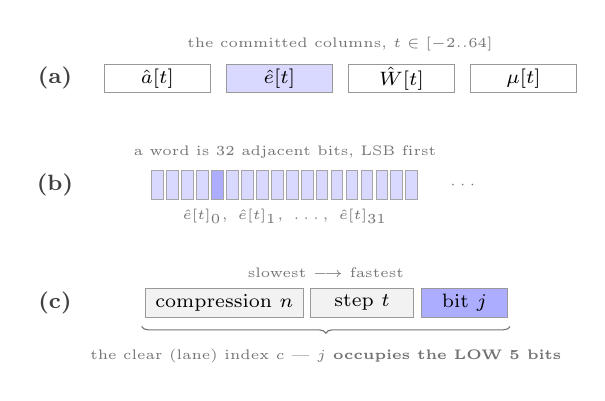
\begin{tikzpicture}[
  font=\scriptsize,
  cel/.style={draw=black!40, minimum width=0.62cm, minimum height=0.36cm,
              inner sep=0pt, line width=0.3pt},
  bitc/.style={draw=black!35, minimum width=0.15cm, minimum height=0.36cm,
              inner sep=0pt, line width=0.25pt},
  hlA/.style={fill=blue!15},
  hlB/.style={fill=blue!32},
  lbl/.style={font=\footnotesize\bfseries, text=black!75},
  dcap/.style={font=\tiny, text=black!55, align=center},
  arr/.style={-{Latex[length=1.8mm]}, draw=black!50, line width=0.5pt},
]
%% Three stacked rows with a left gutter for the panel letters.  A side-by-side
%% layout put the (b) and (c) labels on top of the arrow captions.
\def\GUT{-1.30}

%% ---- (a) the committed columns ----
\begin{scope}[shift={(0,0)}]
  \foreach \i/\lab in {0/{\hat a},1/{\hat e},2/{\hat W},3/{\mu}} {
    \pgfmathsetmacro\bx{\i*1.55}
    \ifnum\i=1
      \node[cel, hlA, minimum width=1.35cm] at (\bx,0) {$\lab[t]$};
    \else
      \node[cel, minimum width=1.35cm] at (\bx,0) {$\lab[t]$};
    \fi
  }
  \node[dcap] at (2.32,0.44) {the committed columns, $t\in[-2..64]$};
  \node[lbl]  at (\GUT,0) {(a)};
\end{scope}

%% ---- (b) one word expanded into its coefficients ----
\begin{scope}[shift={(0,-1.35)}]
  \foreach \k in {0,...,17} {
    \pgfmathsetmacro\bx{\k*0.19}
    \ifnum\k=4
      \node[bitc, hlB] at (\bx,0) {};
    \else
      \node[bitc, hlA] at (\bx,0) {};
    \fi
  }
  \node[dcap] at (3.90,0) {$\cdots$};
  \node[dcap] at (1.62,0.42) {a word is $32$ adjacent bits, LSB first};
  \node[dcap] at (1.62,-0.40) {$\hat e[t]_0,\ \hat e[t]_1,\ \dots,\ \hat e[t]_{31}$};
  \node[lbl]  at (\GUT,0) {(b)};
\end{scope}

%% ---- (c) the flat index ----
\begin{scope}[shift={(0,-2.85)}]
  \node[cel, minimum width=2.0cm, fill=black!5] at (0.85,0) {compression $n$};
  \node[cel, minimum width=1.3cm, fill=black!5] at (2.60,0) {step $t$};
  \node[cel, minimum width=1.1cm, hlB]          at (3.90,0) {bit $j$};
  \node[dcap] at (2.14,0.38) {slowest $\longrightarrow$ fastest};
  \draw[decorate, decoration={brace, amplitude=2.4pt, mirror}, draw=black!55]
    (-0.20,-0.30) -- (4.48,-0.30);
  \node[dcap] at (2.14,-0.68)
    {the clear (lane) index $c$ --- \textbf{$j$ occupies the LOW 5 bits}};
  \node[lbl]  at (\GUT,0) {(c)};
\end{scope}
\end{tikzpicture}
\captionof{figure}{Flattening. The bit position $j$ occupies the \emph{low}
five bits of the clear axis --- not a free choice; see
\cref{rem:layout}.}\label{fig:flatten}
\end{center}

\begin{remark}[Why $j$ must be lowest]\label{rem:layout}
The tap machinery that realises $M$ asserts $g\leq s$: the word group width
$g=5$ must fit inside the clear axis, because $\ROTR$ and $\SHR$ are
implemented as permutations of \emph{clear rows}
\src{src/taps.rs}. Word offsets need $\mathit{off}<2^{s-g}$, and the schedule
reads $\hat W[t{-}16]$, so $s\geq11$; containing a whole per-compression role
block wants $s\geq13$. This is the single layout pin the whole construction
hangs on, and it is the reason the alternative bit-diagonal virtualization path
cannot express SHA-256 at all.
\end{remark}

\subsection{The transpose}\label{sec:committedorder}

The flat order of \cref{fig:flatten} is \emph{not} the committed order. Between
the two sits the one genuine permutation on the entire commit path, and \S2.1's
claim that ``the order is load-bearing'' is really a claim about this step.

Write the flat index as $(\text{fold }b \mid \text{clear }c)$. The commitment
reads the bit matrix \emph{column by column}:
\[
  \underbrace{b\cdot 2^{s} + c}_{\text{flat}}
  \;\longmapsto\;
  \underbrace{c\cdot 2^{t_w} + b}_{\text{committed}},
  \qquad t_w \;=\; \text{row-bit width},
\]
a per-column gather with stride $2^{s}$ --- exactly the transpose of the
$2^{t}\times2^{s}$ bit matrix. \src{src/ligerito.rs}~\code{repack\_leaf\_bits},
target shape documented at \src{src/pcs.rs} as
$M[c][(b\ll\log_2 W)\,|\,j]$.

\begin{warning}[Two readings of \cref{fig:flatten} do not survive it]
\label{warn:transpose}
\Cref{fig:flatten}(b) says ``a word is $32$ adjacent bits''. That is true of the
\emph{flat} order and false of the committed one: after the transpose the $32$
bits of one SHA-256 word differ only in the clear index, so they are strided by
$2^{t_w}$.

The consequence lands on the next figure. A $128$-bit pack window contains
\textbf{at most one bit of any SHA-256 word} --- it is one fixed clear slot read
across $128$ consecutive fold rows, not four adjacent words. A reader who
carries the flat picture forward will conclude that a packed
$\comfield$ element holds four words of the trace. It holds one bit from each of
$128$ different rows.
\end{warning}

\noindent
With that named, the rest of the path is easy to state, because \emph{nothing
else moves}:

\begin{center}\small
\begin{tabular}{@{}llp{0.46\textwidth}@{}}
\toprule
step & moves? & what it is\\
\midrule
transpose      & \textbf{yes} & per-column gather, stride $2^{s}$
                 --- \code{repack\_leaf\_bits}\\
pack to $\comfield$ & no & blocking of a contiguous array\\
interleave     & no & index decomposition; the SoA order already matches\\
rate expansion & no & contiguous replication of the message\\
RS encode      & no & arithmetic in place, lane-wise (additive NTT)\\
\bottomrule
\end{tabular}
\end{center}

\noindent
So the answer to ``where does the reordering happen?'' is: once, here, and never
again. Everything after this line is the same bits in the same order, viewed
through different index decompositions.

\begin{warning}[Which commit path a SHA-256 instance takes is not pinned]
\label{warn:twopaths}
The repository carries \emph{two} layouts --- one placing the bit position on the
fold axis, one on the clear axis with $g=5$ (\cref{rem:layout} describes the
latter) --- and the transpose above belongs to the first. The second commits
packed clear rows directly. Neither builder has a call site under
\code{src/}, \code{examples/}, \code{benches/} or \code{tests/}, and no test
pins the packed-message index map; correctness is enforced only indirectly, by a
ring-switch recombination assertion and end-to-end round trips. So the layout
this section prints is the documented one, not a measured one. A direct test of
the index map would be cheap insurance.
\end{warning}

\subsection{The two axes, and who fixes them}\label{sec:axes}

The transpose above is what splits the witness into a matrix, and that matrix's
shape is a \emph{commitment-time} decision --- fixed by
\code{IntEvalParams}$\{t,s,\text{word\_bits}\}$ before anything is proved. Write
\[
  \begin{gathered}
    \ell = \ellrow\ellcol,\\
    \ellrow = 2^{t_w}\; (\text{row/fold axis}),
    \qquad
    \ellcol = 2^s\; (\text{column/clear axis}).
  \end{gathered}
\]
These are the paper's $\ell_1$ and $\ell_2$, respectively; semantic names are
used from here on. Here $t_w=t+\log_2 W$ --- \code{row\_bit\_vars}, \emph{not} the struct field
\code{ShaF2Layout.tw}, which is a different and smaller quantity ($6$ against
$t=13$ at one shipped layout, so $2^{\mathtt{tw}}=64$ where $\ellrow=8192$). Everything downstream inherits this and nothing
downstream can change it: $\ellrow$ is the number of rows in each grand product in
\cref{step:gkr}, and $\ellcol$ is the number of column integers the prover puts in the
clear at \cref{step:tensor}.

What makes the choice interesting is that \textbf{three unrelated layers each
pin one end of it}, and they very nearly meet:

\begin{center}\small
\begin{tabular}{@{}llp{0.40\textwidth}@{}}
\toprule
bound & from & why\\
\midrule
$t_w\geq7$        & the pack & a $\comfield$ element is $128$ bits, so
                                $128\mid\ellrow$ \src{src/ligerito\_flock.rs}\\
$s\geq13$         & the taps & rotations are permutations of clear rows and
                                need $g\leq s$; a whole per-compression role
                                block wants $s\geq13$ (\cref{rem:layout})\\
$t+W\leq127-q_{\text{bits}}$ & \textbf{the exponent fold}
                  & the honest column sum must not wrap $\ord(g)$; for a
                    $100$-bit prime this is $t+W<28$ \src{src/pcs.rs}\\
\bottomrule
\end{tabular}
\end{center}

\noindent
The third is the one to notice, and it is easy to overstate. It is a
\textbf{soundness} bound arriving from four steps away, so the commitment layout
and the exponent fold of \cref{step:exponent} are not independent choices ---
something neither section says on its own. But it is a \emph{ceiling}, not a
forcing constraint: unsplit ($\ellcol=1$) the single exponent first wraps at
$\ell=2^{29}$, and limb chunking pushes even that to $\ell\approx2^{125}$ at a
cost of $L=\lceil q_{\text{bits}}/c_w\rceil$ parallel forests. The paper
explicitly admits the trivial decomposition $\ellrow=\ell$, $\ellcol=1$.

\textbf{So why split at all? Verifier cost.} The verifier's only
super-logarithmic work is one $\Theta(\ellrow)$ pass --- $2^{t}$ wide fixed-base
exponentiations building the weight table \src{row\_bit\_weights --- src/pcs.rs}
--- and one $\Theta(\ellcol)$ pass over the sent integers. Unsplit that is
$\Theta(\ell)$: a full witness-length sweep, and no succinctness at all. Split,
it is $\Theta(\ellrow+\ellcol)$, minimised near $\sqrt\ell$. Chunking cannot
substitute, because it \emph{multiplies} the verifier by $L$.

Where the shape shows up in cost, then: $\ellcol$ drives \emph{proof size} ---
$L\cdot\ellcol$ integers of $16$ bytes each, about $43\%$ of the whole proof at
$n=26$, $s=13$ --- so a larger $\ellrow$ shrinks the proof. \emph{Prover} time is
$\Theta(\ellrow\ellcol)=\Theta(\ell)$ whichever way the split falls; the forest
evaluates every leaf and every internal node regardless (\cref{step:gkr}).
Every layout in the repository makes $s$ a fixed fraction of $n$ ($\lfloor
2n/5\rfloor$, or $\approx n/2$), so the sent-integer block is
$\Theta(N^{2/5})$--$\Theta(N^{1/2})$: neither constant nor linear in the number
of hashes. \Cref{sec:config} carries the measured numbers.

\subsection{From bits to a root}

\begin{center}
\begin{tikzpicture}[
  font=\scriptsize,
  bitc/.style={draw=black!35, minimum width=0.14cm, minimum height=0.34cm,
              inner sep=0pt, line width=0.25pt},
  fe/.style={draw=black!45, rounded corners=1pt, minimum width=0.88cm,
             minimum height=0.44cm, inner sep=0pt, line width=0.4pt},
  hlO/.style={fill=orange!40},
  hlOl/.style={fill=orange!15},
  lbl/.style={font=\footnotesize\bfseries, text=black!75},
  dcap/.style={font=\tiny, text=black!55, align=center},
  arr/.style={-{Latex[length=1.8mm]}, draw=black!50, line width=0.5pt},
  mk/.style={draw=black!45, circle, minimum size=0.24cm, inner sep=0pt,
             line width=0.35pt},
]
\def\GUT{-1.45}

%% ---- (a) pack ----
\begin{scope}[shift={(0,0)}]
  \foreach \k in {0,...,15} {
    \pgfmathsetmacro\bx{\k*0.14}
    \ifnum\k<5   \node[bitc, hlOl] at (\bx,0) {}; \fi
    \ifnum\k>4 \ifnum\k<11 \node[bitc, hlO] at (\bx,0) {}; \fi\fi
    \ifnum\k>10  \node[bitc, hlOl] at (\bx,0) {}; \fi
  }
  \draw[decorate, decoration={brace, amplitude=2.2pt}, draw=black!60]
    (5*0.14-0.07,0.26) -- (10*0.14+0.07,0.26);
  \node[dcap] at (1.05,0.58) {$128$ consecutive \emph{committed} bits};
  \node[dcap] at (1.05,-0.42) {$\pitwo(\bitsop(\ff))$};
  \node[lbl]  at (\GUT,0) {(a)};

  \draw[arr] (2.45,0) -- node[dcap, above, yshift=1pt]{$\pack$} (3.25,0);

  \node[fe, hlOl] at (3.72,0) {$P_1$};
  \node[fe, hlO]  at (4.66,0) {$P_2$};
  \node[fe, hlOl] at (5.60,0) {$P_3$};
  \node[dcap]     at (6.30,0) {$\cdots$};
  \node[fe, hlOl] at (7.05,0) {$P_{\ell/128}$};
  \node[dcap] at (5.38,-0.44) {$P\in\comfield^{\ell/128}$, \code{LOG\_PACKING}$=7$};
\end{scope}

%% ---- (b) interleave + encode --- POSITION-MAJOR.
%% flock stores codeword[pos * num_ntts + lane]: rows = code positions (a row is
%% one contiguous Merkle leaf), columns = lanes (a column is one RS codeword).
%% The encoder runs DOWN a column; expansion ADDS ROWS.  The earlier drawing had
%% this transposed, which made the leaf a gather -- the thing flock avoids.
%% Every annotation sits OUTSIDE both blocks; labels beside the cells overlapped
%% them, and the log says nothing about that.
\begin{scope}[shift={(0,-2.45)}]
  \foreach \r in {0,1,2} {
    \pgfmathsetmacro\yy{-\r*0.40}
    \foreach \c in {0,1,2,3} {
      \pgfmathsetmacro\bx{\c*0.46}
      \ifnum\r=0 \ifnum\c=1 \node[fe, hlO, minimum width=0.38cm] at (\bx,\yy) {};
        \else \node[fe, hlOl, minimum width=0.38cm] at (\bx,\yy) {}; \fi
      \else \node[fe, hlOl, minimum width=0.38cm] at (\bx,\yy) {}; \fi
    }
  }
  \node[dcap] at (0.69,0.52) {message\\$2^{m_p-k_0}$ positions};
  \draw[arr] (1.95,-0.40) -- (2.60,-0.40);

  \foreach \r in {0,...,5} {
    \pgfmathsetmacro\yy{-\r*0.40}
    \foreach \c in {0,1,2,3} {
      \pgfmathsetmacro\bx{3.05+\c*0.46}
      \ifnum\c=1
        \ifnum\r=0 \node[fe, hlO,  minimum width=0.38cm] at (\bx,\yy) {};
        \else      \node[fe, hlOl, minimum width=0.38cm] at (\bx,\yy) {}; \fi
      \else \node[fe, minimum width=0.38cm, fill=black!5] at (\bx,\yy) {}; \fi
    }
  }
  \node[dcap] at (3.74,0.52) {codeword\\$2^{k_{\mathrm{code}}}$ positions};

  \draw[draw=black!70, line width=0.6pt, rounded corners=1pt]
    (3.05-0.26,-1.20+0.26) rectangle (3.05+3*0.46+0.26,-1.20-0.26);


  \draw[arr] (5.05,0.10) -- (5.05,-2.10);
  \node[dcap, anchor=west] at (5.18,-1.00)
    {additive NTT\\runs \emph{down}\\each lane};

  \node[dcap] at (2.60,-2.62)
    {$2^{k_0}$ lanes, each an independent RS codeword
     ($k_0=\code{initial\_k}$; $16$ by default);\\
     the outlined row is one Merkle leaf --- contiguous in memory};
  \node[lbl]  at (\GUT,-0.40) {(b)};
\end{scope}

%% ---- (c) Merkle ----
\begin{scope}[shift={(2.75,-6.30)}]
  \draw[draw=black!30, line width=0.4pt]
    (0.9,0.30) -- (0.45,-0.10) (0.9,0.30) -- (1.35,-0.10)
    (0.45,-0.10) -- (0.20,-0.52) (0.45,-0.10) -- (0.70,-0.52)
    (1.35,-0.10) -- (1.10,-0.52) (1.35,-0.10) -- (1.60,-0.52);
  \node[mk, fill=green!22] at (0.9,0.30) {};
  \node[mk] at (0.45,-0.10) {}; \node[mk] at (1.35,-0.10) {};
  \node[mk] at (0.20,-0.52) {}; \node[mk] at (0.70,-0.52) {};
  \node[mk] at (1.10,-0.52) {}; \node[mk] at (1.60,-0.52) {};
  \node[dcap] at (0.9,-0.94) {$\mathsf{root}$ (SHA-256); leaf $=$ one row,
     $2^{k_0}$ elements $=2^{k_0}{\cdot}16$ bytes};
  \node[lbl] at (\GUT-2.75,-0.10) {(c)};
\end{scope}
\draw[arr] (3.65,-5.35) -- (3.65,-5.87);
\end{tikzpicture}
\captionof{figure}{Packing, encoding and the root. Orange traces one $128$-bit
window becoming one $\comfield$ element, taking one slot of the message matrix,
and being spread by the encoder \emph{down} its lane. The matrix is drawn
position-major because that is how it is stored: a Merkle leaf is a contiguous
row, and no gather is ever performed.}\label{fig:toroot}
\end{center}

\begin{remark}[The witness does not become one big number]
``Pack the witness into $\comfield$'' invites the wrong picture. Each
\emph{consecutive block of $128$ bits} becomes one field element, so the result
is a \emph{vector} of $\ell/128$ elements; $128$ is a property of the
commitment field, not of the data. And packing never crosses a \emph{column}
boundary, because $128\mid\ellrow$ --- \src{src/ligerito\_flock.rs} asserts
$t+\log_2 W\geq7$. Lanes are a different axis entirely (\cref{warn:lanes}), and
the pack never has to know about them.
\end{remark}

\begin{warning}[A lane is not a compression, and $\ellcol$ is not $N$]
\label{warn:lanes}
Two shape claims that earlier drafts of this section carried are wrong, and both
matter downstream.

\textbf{The lane count is an encoder knob, not the trace.} Interleaving is
$2^{k_0}$-fold with $k_0=\code{initial\_k}$ --- $16$ lanes by default --- and the
lane index is the \emph{low} $k_0$ bits of the packed index, i.e.\ fold-side
coordinates sitting just above the seven the pack absorbed. So a lane is not
``one compression'', and every lane draws entries from every clear column.

\textbf{And $\ellcol$ is the clear-column count $2^{s}$, not $N$.} The
$\mu[\colidx]$ values of \cref{sec:iopp} are one per clear column, and each
grand product runs down the row/fold axis $\ellrow=2^{t_w}$. Mind what this does
and does not say: $\ell=\ellrow\ellcol$ is the \emph{total} committed bit count
and is $\Theta(N)$; only the $\ellcol$ factor is sublinear.  The sent-integer
block must therefore be costed against $2^s$, not against $N$.

Both statements are read off the configuration and commit code rather than
measured, and \cref{warn:twopaths} applies.
\end{warning}

\subsection{Where bit-ness comes from}

\Cref{warn:bitness} asked at which layer the $\bits$ guarantee enters. It enters
\emph{here}, and it is worth being precise because the whole arithmetization
leans on it.

$\pitwo:\Z\to\Ftwo$ is catastrophically lossy on a general integer --- that is
parity collapse, the obstruction F2Z exists to solve. On $\bits$ it is a
\emph{bijection}. So bit-decomposition is not a storage convention: it is the
precondition that makes the one unavoidable $\Z\to\Ftwo$ crossing
information-preserving. A cell of $\ff$ is a bit because the committed object
\emph{is} a bit vector --- there is no representation in which it could be
anything else.

The same restriction buys the exponent fold of \cref{sec:iopp}: $P(Y,Z)=(Y-1)Z+1$
is affine in $Z$ only because $Z\in\bits$.

\begin{remark}[What the root does \emph{not} bind]
The root binds $P$, hence $\bitsop(\ff)$, hence $\ff$ --- \emph{but only given
that $\orc$ is a codeword}, which nothing so far establishes. A cheating prover
can publish a root over an arbitrary vector. All binding is conditional on the
proximity test in \cref{step:proximity}, which is why the commitment claim stays
open in the ledger for the entire protocol rather than being discharged at
commit time.
\end{remark}


\clearpage
\section{The PIOP: collapse and shape the constraint system}\label{sec:piop}

This section is the zero-check.  Its input is the integer relation from
\cref{sec:arith}; its output is one linear claim about the virtual bit witness.
For SHA-256 the relation is linear, so the nonlinear outer sumcheck disappears.
The inner sumcheck remains: the public row collapse produces an arbitrary
coefficient vector, and \cref{step:eqshape} converts it to the separable
$\eq$-shaped vector required by the tensorized F2Z opening.  The interaction is
one row challenge followed by a degree-$2$ sumcheck over the witness-position
variables.

\subsection{Normalize the statement to one witness vector}

The public SHA data must still enter the relation, but it need not be a witness
block.  Let $A_{\xx}$ denote the constraint matrix after substituting the public
message, chaining value, digest, and round constants.  Add one verifier-known
constant coordinate to the source vector,
\[
  \ff^{\circ}=(1,\ff),
\]
and let $M^{\circ}$ contain the constant row, the identity rows for $\ff$, and
the seven XOR families.  Define
\[
  \hh^{\circ}
  =\pitwo^{-1}\!\bigl(M^{\circ}\pitwo(\ff^{\circ})\bigr),
  \qquad
  A_{\xx}^{\circ}\hh^{\circ}=0\quad\text{over }\Z .
\]
The constant column of $A_{\xx}^{\circ}$ carries every affine term created by
substituting $\xx$.  Thus the PIOP witness really is just
\[
  \boxed{\ z=\hh,\qquad A\hh=0,\qquad
  \pitwo(\hh)=M\pitwo(\ff^{\circ})\ },                 \tag{3.1}
\]
where from now on the circles and the subscript $\xx$ are suppressed.  Only the
tail $\ff$ is committed.  The leading $1$ is verifier-known and will reappear as
a known scalar when $M$ is transposed in \cref{step:transpose}.  This
normalization removes the old $(\xx,\ff,\hh)$ concatenation and, with it, the
separate public-input-fold step; it does \emph{not} remove the public input from
the statement.

The two obligations not proved by the zero-check are already fixed.  Commit
time fixed
\[
  C:\quad \orc=\cw{\ff},
\]
and the public virtual map fixes
\[
  H:\quad \pitwo(\hh)=M\pitwo(\ff^{\circ}).
\]
They remain open throughout this section.  The opening IOP will discharge $H$
by the full adjoint of $M$, and $C$ by the final proximity proof.

\paragraph{Indices used below.}
Constraint rows are indexed by
$\beta\in\bits^{\nu}$.  The symbol $\beta$ is deliberately kept separate from
$\rowidx$ and $\colidx$: those two names are reserved for the matrix reshape of
the witness in \cref{sec:iopp}.  Every inner product is annotated by its
ambient field; no inner-product subscript denotes an axis.

\clgreset
\renewcommand{\clgboardtitle}{Open claims}
\clgdef{$\cw{\cdot}$}{$\cw{\ff}=\Enc_{\cC}(\pack(\pitwo(\ff)))$,
  \cref{eq:cw}}

\begin{step*}{Where the PIOP starts}{%
  \clgnew{S}{$A\hh=0$ over $\Z$}%
  \clgnew{C}{$\orc=\cw{\ff}$}%
  \clgnew{H}{$\pitwo(\hh)=M\pitwo(\ff^{\circ})$}%
  \clgnote{S}{$\hh$ is the only PIOP witness vector}%
}
The statement claim $S$ is active.  Claims $C$ and $H$ are standing
obligations: the PIOP carries them but cannot inspect the oracle or prove that a
materialized virtual row came from $M$.
\end{step*}

% =========================================================================
\begin{step}{Multilinearize the constraint rows}{%
  \clgupd{S}{$Q(\beta)=0$ for every $\beta\in\bits^{\nu}$}%
  \clgnote{S}{identity over $\Z$; no challenge and no message}%
}\label{step:mlin}
Pad the $m$ live constraint rows to $2^{\nu}$ and write $A[\beta,*]$ for one
row.  Define the multilinear extension of the residual table:
\[
  Q(Z)
  \defeq
  \sum_{\beta\in\bits^{\nu}}
     \eq(\beta,Z)\,\ipZ{A[\beta,*]}{\hh}.
\]
At a Boolean point, $\eq$ is the Kronecker delta, hence
\[
  A\hh=0
  \quad\Longleftrightarrow\quad
  Q(\beta)=0\quad\text{for every }\beta\in\bits^{\nu}.
\]
This is only a change of notation.  In particular, there is nothing to sum out
yet: the universally quantified row label $\beta$ has merely become the input
of one multilinear polynomial.

\end{step}

% =========================================================================
\begin{step}{Project the integer equations into $\Fq$}{%
  \clgupd{S}{$\bar A\,\pi_q(\hh)=0$ over $\Fq$}%
  \clgnote{S}{$\bar A=\pi_q(A)$; $q=2^{100}-15$ is fixed}%
}\label{step:project}
Reduce the matrix entrywise:
\[
  \bar A\defeq\pi_q(A),
  \qquad
  Q_q(Z)
  \defeq
  \sum_{\beta\in\bits^{\nu}}
    \eq(\beta,Z)\,\ipq{\bar A[\beta,*]}{\pi_q(\hh)}.
\]
All entries of $\hh$ are bits and the nonzero entries of $A$ are signed powers
of two no larger than $2^{35}$.  The public row-wise residual bound is far below
$q$, so reduction cannot turn a nonzero reachable integer residual into zero.

\begin{remark}[Why a fixed $q$ is sound here]\label{warn:fixedq}
The required side condition is
\[
  q>2\max_{\beta}\sum_{\mathsf{pos}}|A[\beta,\mathsf{pos}]|.
\]
For this SHA-256 matrix the right-hand side is below approximately $2^{38}$,
whereas $q\approx2^{100}$.  Therefore projection is injective on every possible
bit-witness residual and introduces zero soundness error.  A redesign of the
arithmetization must recompute this bound.
\end{remark}

\end{step}

% =========================================================================
\begin{step}{Collapse every constraint row at one random point}{%
  \clgdone{S}%
  \clgnew{$E_0$}{$\ipq{\vv}{\pi_q(\hh)}=0$}%
  \clgnote{$E_0$}{$\vv=\bar A^{\!\top}\eq(\cdot,r_{\rm con})$, public}%
}\label{step:collapse}
The verifier samples one point
$r_{\mathrm{con}}\leftarrow\Fq^{\nu}$ and computes
\[
  \vv
  \defeq
  \bar A^{\!\top}\eq(\cdot,r_{\mathrm{con}}),
  \qquad
  \vv[\mathsf{pos}]
  =\sum_{\beta\in\bits^{\nu}}
      \eq(\beta,r_{\mathrm{con}})\bar A[\beta,\mathsf{pos}].
\]

\paragraph{Why evaluation away from the Boolean cube is still zero.}
Let
\[
  e_{\beta}
  \defeq
  \ipq{\bar A[\beta,*]}{\pi_q(\hh)}.
\]
When the constraint claim holds, $e_{\beta}=0$ for every Boolean row label
$\beta$.  Therefore the defining interpolation formula gives
\[
  Q_q(Z)
  =\sum_{\beta\in\bits^{\nu}}\eq(\beta,Z)e_{\beta}
  =\sum_{\beta\in\bits^{\nu}}\eq(\beta,Z)\cdot 0
  =0
  \qquad\text{in }\Fq[Z_1,\ldots,Z_{\nu}].
\]
Thus $Q_q$ is the zero polynomial, not merely a polynomial that happens to
vanish at the Boolean points, and consequently
$Q_q(r_{\mathrm{con}})=0$ for \emph{every}
$r_{\mathrm{con}}\in\Fq^{\nu}$.  Multilinearity is load-bearing here: a general
polynomial such as $Z(Z-1)$ can vanish on the Boolean cube without vanishing
away from it, but $Q_q$ is by construction the unique multilinear extension of
the residual table.

For any witness, whether valid or not, reassociating the sums gives
\[
  Q_q(r_{\mathrm{con}})
  =\sum_{\beta}\eq(\beta,r_{\mathrm{con}})
       \ipq{\bar A[\beta,*]}{\pi_q(\hh)}
  =\ipq{\vv}{\pi_q(\hh)}.
\]
The verifier replaces the full row claim by the randomized scalar claim
\[
  \boxed{\ipq{\vv}{\pi_q(\hh)}=0}.             \tag{$E_0$}
\]
The prover sends nothing.  If a nonzero multilinear residual table is claimed
to be zero, the random evaluation accepts with probability at most
$\nu/|\Fq|$.

\paragraph{What the row collapse does --- and does not do.}
There is no reason to sumcheck the row label $\beta$: $A$ is public and the
witness occurs linearly, so the complete $\beta$-sum moves onto $A$ and becomes
the public vector $\vv$.  But this does \emph{not} make $\vv$ a tensor product
across the later row/column layout.  The next step sumchecks the
\emph{witness-position} variables; confusing those two index sets is exactly
what allowed the missing reduction to go unnoticed.

For $N$ copies of the same circuit, the circuit-dependent portion of this pass
factors through the one-compression matrix.  Public-data-dependent coefficients
still have to be read; the h-only normalization relocates that work into the
construction of $A_{\xx}$ rather than pretending public I/O is free.

\end{step}

% =========================================================================
\begin{step}{Sumcheck the inner product into an evaluation-shaped claim}{%
  \clgdone{$E_0$}%
  \clgnew{$E_{\rm eq}$}{$c\,\mle{h_q}(r_h)=\tau$}%
  \clgnote{$E_{\rm eq}$}{weights are $c\,\eq(\cdot,r_h)$, hence separable}%
}\label{step:eqshape}
Pad $\hh$ and $\vv$ with zeros to a common length $2^{d_h}$, write
$h_q\defeq\pi_q(\hh)$, and let $\mle{\vv}$ and $\mle{h_q}$ denote their
multilinear extensions.  The claim from \cref{step:collapse} is
\[
  0
  =\sum_{p\in\bits^{d_h}}\vv[p]h_q[p]
  =\sum_{p\in\bits^{d_h}}\mle{\vv}(p)\mle{h_q}(p).    \tag{3.2}\label{eq:eqshape-start}
\]
Run the standard degree-$2$ sumcheck on \eqref{eq:eqshape-start}.  At round
$i$, after challenges $r_1,\ldots,r_{i-1}$, the prover sends
\[
\begin{aligned}
  g_i(T)
  ={}&\!\!\sum_{x_{i+1},\ldots,x_{d_h}\in\bits}
    \mle{\vv}(r_1,\ldots,r_{i-1},T,x_{i+1},\ldots,x_{d_h})\\[-2pt]
   &\hspace{2.2cm}\cdot
    \mle{h_q}(r_1,\ldots,r_{i-1},T,x_{i+1},\ldots,x_{d_h}).
\end{aligned}
\]
The verifier checks
\[
  g_i(0)+g_i(1)=s_{i-1},
\]
samples $r_i\leftarrow\Fq$, and sets $s_i=g_i(r_i)$, starting from
$s_0=0$.  After $d_h$ rounds, put
\[
  r_h=(r_1,\ldots,r_{d_h}),
  \qquad \tau=s_{d_h},
  \qquad c=\mle{\vv}(r_h),
\]
where $c$ is public because $\vv$ is public.  The terminal relation is
\[
  \tau=c\,\mle{h_q}(r_h)
      =\ipq{c\,\eq(\cdot,r_h)}{\pi_q(\hh)}.
\]
Thus the sumcheck replaces the arbitrary coefficient vector by the rank-one
evaluation vector:
\[
  \boxed{
  E_{\rm eq}:\quad
  \ipq{c\,\eq(\cdot,r_h)}{\pi_q(\hh)}=\tau.}         \tag{3.3}\label{eq:eqshape-end}
\]
Keeping the scalar $c$ in the coefficient vector avoids division and remains
valid even when $c=0$.  Equivalently, one may fuse
\cref{step:collapse,step:eqshape} into a Spartan-style matrix sumcheck; the
contracted-$\vv$ presentation is the minimal change because the verifier
already performs the sparse public matrix--vector pass.

\end{step}

\subsection{PIOP handoff and error budget}

The SHA-256 PIOP has exactly four moves:
\[
  \begin{aligned}
  A\hh=0\text{ over }\Z
  &\xRightarrow{\text{multilinearize}}
    Q|_{\bits^{\nu}}=0
   \xRightarrow{\pi_q}
    \bar A\pi_q(\hh)=0,\\
  &\xRightarrow{r_{\mathrm{con}}}
    E_0
   \xRightarrow{\text{degree-2 sumcheck}}
    E_{\rm eq}.
  \end{aligned}
\]
Projection contributes no error under \cref{warn:fixedq}.  Evaluating the
multilinear residual contributes at most $\nu/|\Fq|$, and the degree-$2$
sumcheck contributes at most $2d_h/|\Fq|$.  No ideal check,
polynomial-basis evaluation, public-input fold, or bit-decomposition remains.


\clearpage
\section{The opening IOP}\label{sec:iopp}

The PIOP hands this section exactly three open claims:
\[
  E_{\rm eq}:\ipq{c\,\eq(\cdot,r_h)}{\pi_q(\hh)}=\tau,
  \qquad
  H:\pitwo(\hh)=M\pitwo(\ff^{\circ}),
  \qquad
  C:\orc=\cw{\ff}.
\]
The virtual witness $\hh$ is already a bit vector, so there is no
bit-decomposition step for SHA-256.  Crucially, the PIOP has already changed the
arbitrary coefficient vector $\vv=\bar A^{\!\top}\eq(\cdot,r_{\rm con})$ into
the evaluation-shaped vector $c\,\eq(\cdot,r_h)$.  The opening may now reshape
that vector without assuming a tensor factorisation of $\vv$.

\subsection{Axes and fields}

The committed vector $\ff$ already has the commitment-time matrix view
$F\defeq\operatorname{reshape}(\ff)$ from \cref{sec:commit}.  For the virtual
vector $\hh$, pad to a rectangular power-of-two layout and set
\[
  \begin{gathered}
    \Rows=\bits^{\drow},\qquad \Cols=\bits^{\dcol},\\
    \ellrow=2^{\drow},\qquad
    \ellcol=2^{\dcol},\qquad
    \ellrow\ellcol=2^{d_h}\geq|\hh|,
    \qquad d_h=\drow+\dcol.
  \end{gathered}
\]
The implementation calls these dimensions $\ell_1$ and $\ell_2$; this section
uses the semantic names $\ellrow$ and $\ellcol$.  Reshape the virtual vector as
\[
  H[\rowidx,\colidx]
  =\hh[\colidx\ellrow+\rowidx].                 \tag{4.1}\label{eq:reshape}
\]
The row/fold index is the fastest-moving coordinate, so each
$H[*,\colidx]$ is contiguous and a $128$-bit pack never crosses a column
boundary.  Split the sumcheck point according to exactly these coordinates,
\[
  r_h=(r_{\rm row},r_{\rm col}),
  \qquad
  r_{\rm row}\in\Fq^{\drow},\quad
  r_{\rm col}\in\Fq^{\dcol}.
\]
The equality polynomial factors over a concatenated point:
\[
  \eq\bigl((\rowidx,\colidx),r_h\bigr)
  =\eq(\rowidx,r_{\rm row})\eq(\colidx,r_{\rm col}).
\]
Define the two public weight vectors
\[
  v_{\rm row}[\rowidx]\defeq\eq(\rowidx,r_{\rm row}),
  \qquad
  v_{\rm col}[\colidx]\defeq c\,\eq(\colidx,r_{\rm col}).
\]
Then the PIOP boundary is exactly
\[
  E_{\rm eq}:
  \sum_{\rowidx\in\Rows}\sum_{\colidx\in\Cols}
     v_{\rm row}[\rowidx]v_{\rm col}[\colidx]\,
     \pi_q(H[\rowidx,\colidx])=\tau
  \quad\text{in }\Fq .                         \tag{4.2}
\]
This separation is an identity of the equality polynomial.  It is the output
of \cref{step:eqshape}, not a property assumed of the original $\vv$.
\begin{center}
\small
\(
  \underbrace{
    \operatorname{reshape}\!\left(
      \bar A^{\!\top}\eq(\cdot,r_{\rm con})
    \right)
  }_{\text{usually rank \(>1\)}}
  \quad
  \xRightarrow{\text{\cref{step:eqshape}: sumcheck}}
  \quad
  \underbrace{
    \bigl[\eq(\rowidx,r_{\rm row})\bigr]_{\rowidx}\,
    \bigl[c\,\eq(\colidx,r_{\rm col})\bigr]_{\colidx}^{\!\top}
  }_{\text{rank one for every split}} .
\)
\end{center}
The names $\rowidx$ and $\colidx$ always denote the matrix axes in
\eqref{eq:reshape}.  Inner products instead advertise their field:
$\ipq{\cdot}{\cdot}$, $\ipZ{\cdot}{\cdot}$, or
$\ipC{\cdot}{\cdot}$.

The field path is
\[
  \Fq\ \xrightarrow{\text{canonical lift}}\ \Z
  \ \xrightarrow{a\mapsto\gen^a}\ \comfield^{\times}
  \ \xrightarrow{\text{linear opening}}\ \comfield.
\]

% =========================================================================
\begin{step}{Reshape and send the column folds as integers}{%
  \clgdone{$E_{\rm eq}$}%
  \clgnew{T}{$\mu[\colidx]=\ipZ{\gam}{H[*,\colidx]}$}%
  \clgnote{T}{$\rowidx$ is summed; one integer remains per $\colidx$}%
}\label{step:tensor}
The core opening interface needs public weights that separate across the two
axes.  The preceding sumcheck guarantees exactly that form.  Canonically lift
its row coefficients from $\Fq$ to integers,
\[
  \gam[\rowidx]
  \defeq\pi_{\mathrm{can}}^{-1}
     \bigl(v_{\mathrm{row}}[\rowidx]\bigr)\in[0,q-1].
\]
For every fixed column, the prover sends the integer
\[
  \boxed{
  \mu[\colidx]
  \defeq
  \ipZ{\gam}{H[*,\colidx]}
  =\sum_{\rowidx\in\Rows}
       \gam[\rowidx]H[\rowidx,\colidx] .}       \tag{4.3}\label{eq:mucol}
\]
This dot product runs \emph{down the row axis} of one fixed column, and it runs
over $\Z$.  The verifier checks the original field claim by reducing the sent
integers modulo $q$:
\[
  \boxed{\ipq{v_{\mathrm{col}}}{\pi_q(\bm\mu)}=\tau.}  \tag{4.4}\label{eq:murecombine}
\]
Equations \eqref{eq:mucol} and \eqref{eq:murecombine} are exactly
$E_{\rm eq}$ written column by column.

\begin{center}
\begin{tikzpicture}[
  font=\scriptsize,
  cell/.style={draw=black!38, minimum width=0.48cm, minimum height=0.38cm,
               inner sep=0pt, line width=0.3pt},
  arr/.style={-{Latex[length=1.8mm]}, draw=black!55},
  vcap/.style={font=\tiny, text=black!60, align=center},
]
  \node[vcap,anchor=east] at (-0.42,1.55) {$\ff\in\bits^{|\ff|}$};
  \node (fflat) at (0.02,1.55)
    {$\begin{bmatrix}f_0\\f_1\\[-2pt]\vdots\\[-2pt]f_{|\ff|-1}\end{bmatrix}$};
  \node[vcap,anchor=east] at (-0.42,-0.15) {$\hh\in\bits^{|\hh|}$};
  \node (hflat) at (0.02,-0.15)
    {$\begin{bmatrix}h_0\\h_1\\[-2pt]\vdots\\[-2pt]h_{|\hh|-1}\end{bmatrix}$};
  \draw[arr] (fflat.east) -- node[vcap,above]{reshape} (1.65,1.55);
  \draw[arr] (hflat.east) -- node[vcap,above]{reshape} (1.65,-0.15);

  \begin{scope}[shift={(2.20,1.95)}]
    \foreach \r in {0,...,2}{
      \foreach \c in {0,...,4}{
        \node[cell,fill=blue!8] at (0.50*\c,-0.40*\r) {};
      }
    }
    \node[vcap] at (1.0,0.42) {$F$};
  \end{scope}

  \begin{scope}[shift={(2.20,0.25)}]
    \foreach \r in {0,...,2}{
      \foreach \c in {0,...,4}{
        \ifnum\c=2
          \node[cell,fill=orange!35] at (0.50*\c,-0.40*\r) {$h$};
        \else
          \node[cell,fill=orange!8] at (0.50*\c,-0.40*\r) {};
        \fi
      }
    }
    \node[vcap] at (1.0,0.42) {$H$};
    \draw[orange!75!black,rounded corners=1pt,line width=0.8pt]
      (0.73,0.22) rectangle (1.27,-1.02);
  \end{scope}

  \draw[arr,orange!75!black] (3.20,-0.85) -- (3.20,-1.35);
  \node[draw=orange!65!black,rounded corners=2pt,fill=orange!10,
        minimum height=0.58cm] (mu) at (3.20,-1.70)
    {$\mu[\colidx]=\ipZ{\gam}{H[*,\colidx]}$};
  \node[vcap,anchor=west,text width=3.25cm] at (5.15,-1.70)
    {fix one column; sum over $\rowidx$;\\the inner product is over $\Z$};
  \node[vcap,anchor=west,text width=3.25cm] at (5.15,1.55)
    {sumcheck weights:\\row $\eq(\cdot,r_{\rm row})\mapsto\gam$;\\
     column $c\,\eq(\cdot,r_{\rm col})$};
  \node[vcap] at (3.20,-2.35)
    {repeat independently for all $\ellcol$ columns};
\end{tikzpicture}
\captionof{figure}{The committed vector $\ff$ and virtual vector $\hh$ are
reshaped in their respective layouts into the data matrices $F$ and $H$.
The original public vector $\vv$ is not being factorised here:
\cref{step:eqshape} has already replaced it by the rank-one equality weights
$\eq(\cdot,r_{\rm row})$ and $c\,\eq(\cdot,r_{\rm col})$.
Each $\mu[\colidx]$ is a column fold: the selected column is fixed while the
sum runs over the row axis.}\label{fig:columnfold}
\end{center}

\begin{warning}[The integer messages need an explicit range check]
\label{warn:mujrange}
The field check \eqref{eq:murecombine} fixes $\mu[\colidx]$ only modulo $q$, while the next
step fixes $\gen^{\mu[\colidx]}$ only modulo $\ord(\gen)$.  Therefore the
verifier must reject unless
\[
  0\leq\mu[\colidx]\leq\ellrow(q-1),
  \qquad
  \ellrow(q-1)<\ord(\gen).
\]
The implementation performs this range check and verifies that $\gen$ is
primitive.  Without it, CRT lets a prover alter the field value while
preserving the exponent claim.
\end{warning}

\begin{warning}[Why the evaluation-shaping sumcheck is load-bearing]
\label{warn:rank1}
One cannot skip \cref{step:eqshape} and simply declare the reshaped matrix
$V=\operatorname{reshape}(\vv)$ to be rank one.  In general
$\vv=\bar A^{\!\top}\eq(\cdot,r_{\rm con})$ has no such factorisation; for the
shipped fold/clear splits its measured ranks on a schedule-shaped $A_0$ are
$1,2,4,4,3,2$ as $s-g$ ranges from $0$ to $5$.

The sumcheck fixes this for every axis split: its output coefficient is
$c\,\eq(\cdot,r_h)$, and equality factors exactly over
$r_h=(r_{\rm row},r_{\rm col})$.  A different, more expensive repair would be
to decompose the original table as
\[
  V[\rowidx,\colidx]
  =\sum_{a=1}^{r}v_{\mathrm{row}}^{(a)}[\rowidx]
        v_{\mathrm{col}}^{(a)}[\colidx],
\]
then run the integer-fold, forest, and GKR path for $r$ weight families.
Treating $r=1$ without either repair is a completeness error.
\end{warning}

\end{step}

% =========================================================================
\begin{step}{Move each integer column fold into an exponent}{%
  \clgdone{T}%
  \clgnew{P}{$\prod_{\rowidx}L_d[\rowidx,\colidx]=\gen^{\mu[\colidx]}$}%
  \clgnote{P}{one product per column, all in $\comfield$}%
}\label{step:exponent}
Fix a large-order generator $\gen\in\comfield^{\times}$ and define one leaf for
each matrix entry:
\[
  L_{\drow}[\rowidx,\colidx]
  \defeq
  1+\bigl(\gen^{\gam[\rowidx]}-1\bigr)
       \pitwo(H[\rowidx,\colidx]).                \tag{4.5}\label{eq:leafdef}
\]
Because $H[\rowidx,\colidx]$ is a bit, the leaf is $1$ when the bit is zero and
$\gen^{\gam[\rowidx]}$ when it is one.  Therefore, for every fixed column,
\[
  \boxed{
  \prod_{\rowidx\in\Rows}L_{\drow}[\rowidx,\colidx]
  =\gen^{\sum_{\rowidx}\gam[\rowidx]H[\rowidx,\colidx]}
  =\gen^{\mu[\colidx]}.}                         \tag{4.6}
\]
The product iterates over $\rowidx$; $\colidx$ selects which of the
$\ellcol$ products is being proved.  This is not a sumcheck.  It is the
algebraic bridge from addition over $\Z$ to multiplication in
$\comfield^{\times}$.

\end{step}

% =========================================================================
\begin{step}{Reduce all column products with one merged GKR forest}{%
  \clgdone{P}%
  \clgnew{L}{$e_{\drow}+1=\sum_{\rowidx,\colidx}\!R\,\pitwo(H)$}%
  \clgnote{L}{one leaf-boundary claim over $\comfield$}%
}\label{step:gkr}
There is one product tree for every column, but the trees are proved as a
single forest.  At level $k$, where the root level is $k=0$ and the leaves are
$k=\drow$, use
\[
  \rowprefix\in\bits^k,\qquad \colidx\in\Cols,
\]
and define the recursion
\[
  \boxed{
  L_k[\rowprefix,\colidx]
  =L_{k+1}[\rowprefix\Vert0,\colidx]\,
   L_{k+1}[\rowprefix\Vert1,\colidx].}            \tag{4.7}
\]
The root table is public from Step 5's integers:
\[
  L_0[\colidx]=\gen^{\mu[\colidx]}.
\]
The verifier samples $\zcol^{(0)}\in\comfield^{\dcol}$ and starts from
\[
  E_0^{\mathrm{GKR}}:\quad
  \widetilde L_0(\zcol^{(0)})=e_0,
  \qquad
  e_0=\sum_{\colidx\in\Cols}
       \eq(\colidx,\zcol^{(0)})\gen^{\mu[\colidx]}.
\]

\paragraph{The claim proved at every level.}
Suppose level $k$ starts with
\[
  E_k^{\mathrm{GKR}}:\quad
  \widetilde L_k(\zrow^{(k)},\zcol^{(k)})=e_k,
  \qquad \zrow^{(k)}\in\comfield^k.
\]
The layer sumcheck proves
\begin{align}
  e_k
  ={}&\sum_{\rowprefix\in\bits^k}
      \sum_{\colidx\in\Cols}
      \eq(\rowprefix,\zrow^{(k)})
      \eq(\colidx,\zcol^{(k)})                         \notag\\[-2pt]
     &\hspace{2.4cm}\cdot
      L_{k+1}[\rowprefix\Vert0,\colidx]
      L_{k+1}[\rowprefix\Vert1,\colidx].              \tag{4.8}\label{eq:gkrlayer}
\end{align}
The implementation realizes \eqref{eq:gkrlayer} as two consecutive
degree-$3$ sumchecks.

\paragraph{Which variables are sumchecked at depth $k$.}
Write a complete leaf-row index as
$x=(x_1,\ldots,x_{\drow})$.  A node at depth $k$ retains only the
already-exposed prefix $x_{\leq k}=(x_1,\ldots,x_k)$.  Therefore the first of
the two sumchecks, the row-prefix phase, uses exactly the iteration variables
\[
  X=(X_1,\ldots,X_k)\in\bits^k,
\]
not the unexposed suffix $(x_{k+1},\ldots,x_{\drow})$.  It consequently has
$k$ rounds: none at the root, one at depth $1$, and one additional round at
each deeper multiplication layer.  The child arguments $X\Vert0$ and
$X\Vert1$ append the next row coordinate.

For this row-prefix sumcheck, define the
column-contracted degree-$2$ polynomial
\[
  G_k(X)
  \defeq
  \sum_{\colidx\in\Cols}
    \eq(\colidx,\zcol^{(k)})
    \mle{L_{k+1}}(X,0,\colidx)
    \mle{L_{k+1}}(X,1,\colidx).
\]
The row-prefix sumcheck starts from
\[
  e_k=\sum_{\rowprefix\in\bits^k}
       \eq(\rowprefix,\zrow^{(k)})G_k(\rowprefix).
                                                        \tag{4.8a}
\]
After its row-prefix challenges fix
$r_{\mathrm{row}}^{(k)}$, let
$s_k=G_k(r_{\mathrm{row}}^{(k)})$.  If
$e_{k,\mathrm{row}}^{\mathrm{end}}$ is this sumcheck's terminal value, the
verifier checks
\[
  e_{k,\mathrm{row}}^{\mathrm{end}}
  =\eq(r_{\mathrm{row}}^{(k)},\zrow^{(k)})s_k,
\]
and the column-index sumcheck starts from
\[
  s_k=\sum_{\colidx\in\Cols}
       \eq(\colidx,\zcol^{(k)})
       E_k[\colidx]O_k[\colidx],                       \tag{4.8b}
\]
where
\[
  E_k[\colidx]
   =\widetilde L_{k+1}(r_{\mathrm{row}}^{(k)},0,\colidx),
  \qquad
  O_k[\colidx]
   =\widetilde L_{k+1}(r_{\mathrm{row}}^{(k)},1,\colidx).
\]
Thus the two groups of iteration variables are:
\[
  \underbrace{k\text{ coordinates of }\rowprefix}_{\text{row-prefix sumcheck}}
  \qquad\text{then}\qquad
  \underbrace{\dcol\text{ coordinates of }\colidx}_{\text{column-index sumcheck}}.
\]
The row-prefix sumcheck is empty at the root.  The column-index sumcheck is what
merges all columns; without it, the prover would expose one child pair per
column at every level.

At the end of the level, the verifier has child values
\[
  a_k=\widetilde L_{k+1}(r_{\mathrm{row}}^{(k)},0,
                         r_{\mathrm{col}}^{(k)}),
  \qquad
  b_k=\widetilde L_{k+1}(r_{\mathrm{row}}^{(k)},1,
                         r_{\mathrm{col}}^{(k)}).
\]
If $e_{k,\mathrm{col}}^{\mathrm{end}}$ is the column-index sumcheck's terminal
value, the verifier checks
\[
  e_{k,\mathrm{col}}^{\mathrm{end}}
  =\eq(r_{\mathrm{col}}^{(k)},\zcol^{(k)})a_kb_k.
\]
Only then does the transcript absorb $(a_k,b_k)$ and sample
$\chi_k\in\comfield$, folding the pair into the next boundary claim:
\[
  \boxed{
  \begin{aligned}
  \zrow^{(k+1)}&=(r_{\mathrm{row}}^{(k)},\chi_k),\\
  \zcol^{(k+1)}&=r_{\mathrm{col}}^{(k)},\\
  e_{k+1}&=(1-\chi_k)a_k+\chi_k b_k,\\
  E_{k+1}^{\mathrm{GKR}}&:
    \widetilde L_{k+1}(\zrow^{(k+1)},\zcol^{(k+1)})=e_{k+1}.
  \end{aligned}}                                      \tag{4.9}
\]
This is the recursive relation: each level consumes one claim about $L_k$ and
creates one claim about $L_{k+1}$.

\Cref{fig:gkr-depth4} shows the complete descent for a depth-$4$ example.  The
tree is representative: the row-prefix sumcheck moves within all $2^s$ trees,
whereas the column-index sumcheck is the horizontal contraction that merges
their column index.  In \eqref{eq:gkrlayer}, $\rowprefix\Vert b$ appends the
newly exposed top coordinate.  The figure uses recursive tree order for
legibility, not the low-bit-first flat-table order used by the implementation.

\begin{center}
\begin{tikzpicture}[
  x=1cm,
  y=1cm,
  font=\scriptsize,
  levelband/.style={fill=blue!3, rounded corners=1pt},
  treeedge/.style={draw=black!25, line width=0.35pt},
  treenode/.style={circle, draw=black!42, fill=black!4,
                   minimum size=2.8mm, inner sep=0pt, line width=0.35pt},
  leafnode/.style={treenode, minimum size=1.8mm, fill=orange!9},
  claim/.style={draw=blue!55!black, fill=blue!4, rounded corners=1.5pt,
                minimum width=7.15cm, minimum height=0.42cm,
                inner sep=1.1pt, line width=0.45pt},
  rowsc/.style={draw=blue!55!black, fill=blue!10, rounded corners=1.2pt,
                minimum width=2.20cm, minimum height=0.48cm,
                align=center, inner sep=1pt, line width=0.35pt},
  colsc/.style={draw=orange!70!black, fill=orange!12, rounded corners=1.2pt,
                minimum width=2.45cm, minimum height=0.48cm,
                align=center, inner sep=1pt, line width=0.35pt},
  linefold/.style={draw=black!45, fill=black!4, rounded corners=1.2pt,
                   minimum width=1.55cm, minimum height=0.48cm,
                   align=center, inner sep=1pt, line width=0.35pt},
  claimarr/.style={-{Latex[length=1.5mm]}, draw=blue!50!black,
                   line width=0.45pt},
  tinyarr/.style={-{Latex[length=1.2mm]}, draw=black!45,
                   line width=0.35pt},
  rowdetail/.style={draw=blue!55!black, fill=blue!7, rounded corners=1.5pt,
                    text width=3.80cm, minimum height=1.68cm,
                    align=center, inner sep=3pt, line width=0.4pt},
  coldetail/.style={draw=orange!70!black, fill=orange!8,
                    rounded corners=1.5pt, text width=3.75cm,
                    minimum height=1.68cm, align=center,
                    inner sep=3pt, line width=0.4pt},
  folddetail/.style={draw=black!45, fill=black!3, rounded corners=1.5pt,
                     text width=3.35cm, minimum height=1.68cm,
                     align=center, inner sep=3pt, line width=0.4pt},
  boundary/.style={draw=orange!70!black, fill=orange!7,
                   rounded corners=1.5pt, align=center,
                   inner sep=3pt, line width=0.45pt},
  dcap/.style={font=\tiny, text=black!58, align=center},
]

% One continuous swimlane: every level table is horizontally aligned with the
% verifier claim about that table.  Operations in the gap reduce that claim to
% the claim on the next level.
\node[dcap, text width=4.1cm] at (2.13,0.70)
  {one representative column tree; the whole tree is repeated $2^s$ times};
\node[dcap, text width=7.15cm] at (8.28,0.70)
  {each level claim is followed by its row-prefix sumcheck, column-index sumcheck,
   and line fold, side by side};

\draw[draw=black!22, dashed, rounded corners=2pt, line width=0.35pt]
  (0.10,0.30) rectangle (4.22,-4.62);
\node[dcap, fill=white, inner sep=0.7pt] at (2.16,-4.62)
  {one complete product tree};

\foreach \lev in {0,...,4} {
  \pgfmathtruncatemacro{\numnodes}{2^\lev}
  \pgfmathtruncatemacro{\lastnode}{\numnodes-1}
  \pgfmathsetmacro{\yy}{-1.10*\lev}
  \path[levelband] (0.18,\yy-0.17) rectangle (4.14,\yy+0.17);
  \foreach \idx in {0,...,\lastnode} {
    \pgfmathsetmacro{\xx}{0.24+3.84*(\idx+0.5)/\numnodes}
    \coordinate (gkr-\lev-\idx) at (\xx,\yy);
  }
  \ifnum\lev=4
    \node[dcap, anchor=east] at (0.06,\yy) {$L_4=\Lambda$};
  \else
    \node[dcap, anchor=east] at (0.06,\yy) {$L_{\lev}$};
  \fi
}

% Recursive visual order keeps the binary tree legible.  The surrounding prose
% states that the implementation's flat tables instead use low-bit-first order.
\foreach \lev in {0,...,3} {
  \pgfmathtruncatemacro{\numnodes}{2^\lev}
  \pgfmathtruncatemacro{\lastnode}{\numnodes-1}
  \pgfmathtruncatemacro{\childlev}{\lev+1}
  \foreach \idx in {0,...,\lastnode} {
    \pgfmathtruncatemacro{\leftchild}{2*\idx}
    \pgfmathtruncatemacro{\rightchild}{2*\idx+1}
    \draw[treeedge] (gkr-\lev-\idx) -- (gkr-\childlev-\leftchild);
    \draw[treeedge] (gkr-\lev-\idx) -- (gkr-\childlev-\rightchild);
  }
}

\foreach \lev in {0,...,4} {
  \pgfmathtruncatemacro{\numnodes}{2^\lev}
  \pgfmathtruncatemacro{\lastnode}{\numnodes-1}
  \foreach \idx in {0,...,\lastnode} {
    \ifnum\lev=4
      \node[leafnode] at (gkr-\lev-\idx) {};
    \else
      \node[treenode] at (gkr-\lev-\idx) {};
    \fi
  }
}

\draw[-{Latex[length=1.7mm]}, draw=black!38, line width=0.45pt]
  (-0.36,-4.22) -- (-0.36,-0.18);
\node[dcap, rotate=90, anchor=center] at (-0.68,-2.20)
  {products computed upward};

% Claims live at the same heights as the product-tree levels.
\node[claim] (E0) at (8.28, 0.00)
  {$E_0^{\mathrm{GKR}}:\ \mle{L_0}(\zcol^{(0)})=e_0$};
\node[claim] (E1) at (8.28,-1.10)
  {$E_1^{\mathrm{GKR}}:\ \mle{L_1}(\zrow^{(1)},\zcol^{(1)})=e_1$};
\node[claim] (E2) at (8.28,-2.20)
  {$E_2^{\mathrm{GKR}}:\ \mle{L_2}(\zrow^{(2)},\zcol^{(2)})=e_2$};
\node[claim] (E3) at (8.28,-3.30)
  {$E_3^{\mathrm{GKR}}:\ \mle{L_3}(\zrow^{(3)},\zcol^{(3)})=e_3$};
\node[claim] (E4) at (8.28,-4.40)
  {$E_4^{\mathrm{GKR}}:\ \mle{L_4}(\zrow^{(4)},\zcol^{(4)})=e_4$};

\foreach \k/\next/\rowrounds/\midy in {
  0/1/0/-0.55,
  1/2/1/-1.65,
  2/3/2/-2.75,
  3/4/3/-3.85} {
  \node[rowsc] (R\k) at (5.70,\midy)
    {row-prefix sumcheck\\$\rowrounds$ rounds};
  \node[colsc] (C\k) at (8.28,\midy)
    {column-index sumcheck\\$s$ rounds};
  \node[linefold] (X\k) at (10.82,\midy)
    {$\chi_{\k}$ line fold};
  \draw[claimarr] (E\k.south west) -- (R\k.north west);
  \draw[tinyarr] (R\k) -- (C\k);
  \draw[tinyarr] (C\k) -- (X\k);
  \draw[claimarr] (X\k.south east) -- (E\next.north east);
}

% Light guides make the level-table / claim correspondence explicit without
% implying that a single selected tree path is being verified.
\foreach \lev in {0,...,4} {
  \draw[draw=black!20, densely dotted, line width=0.3pt]
    (4.22,-1.10*\lev) -- (E\lev.west);
}

% Expand one transition into its exact three consecutive relations.  The boxes
% are horizontal because these are stages of one claim reduction, not functions
% named A and B.
\node[rowdetail] (rowdetail) at (2.05,-6.30) {%
  \textbf{Row-prefix sumcheck} \ ($k$ rounds)\\[2pt]
  $\begin{aligned}
    e_k&=\displaystyle\sum_{x\in\bits^k}
      \eq(x,\zrow^{(k)})\\[-1pt]
      &\qquad\cdot G_k(x),\\[2pt]
    e_{k,\mathrm{row}}^{\mathrm{end}}
      &=\eq(r_{\mathrm{row}}^{(k)},\zrow^{(k)})s_k
  \end{aligned}$
};

\node[coldetail] (coldetail) at (6.25,-6.30) {%
  \textbf{Column-index sumcheck} \ ($s$ rounds)\\[2pt]
  $\begin{aligned}
    s_k&=\displaystyle\sum_{c\in\bits^s}
      \eq(c,\zcol^{(k)})\\[-1pt]
      &\qquad\cdot E_k(c)O_k(c),\\[2pt]
    e_{k,\mathrm{col}}^{\mathrm{end}}
      &=\eq(r_{\mathrm{col}}^{(k)},\zcol^{(k)})a_kb_k
  \end{aligned}$
};

\node[folddetail] (folddetail) at (10.34,-6.30) {%
  \textbf{Absorb the child pair; then fold}\\[2pt]
  $\begin{gathered}
    e_{k+1}=a_k+\chi_k(a_k+b_k),\\[2pt]
    \zrow^{(k+1)}=(r_{\mathrm{row}}^{(k)},\chi_k),\\[1pt]
    \zcol^{(k+1)}=r_{\mathrm{col}}^{(k)}
  \end{gathered}$
};

\draw[claimarr] (rowdetail) -- (coldetail);
\draw[claimarr] (coldetail) -- (folddetail);

\node[boundary, text width=12.05cm] at (6.14,-8.62) {%
  $\displaystyle
  \begin{aligned}
    e_4+1
      &=\sum_{i\in\bits^4}\sum_{c\in\bits^s}
        \eq(i,\zrow^{(4)})\eq(c,\zcol^{(4)})
        \bigl(\gen^{\gam[i]}-1\bigr)\pitwo(H[i,c])\\[-1pt]
      &\hspace{5.3cm}\longrightarrow\quad
        \text{row-only pre-sumcheck}.
  \end{aligned}$
};
\end{tikzpicture}
\captionof{figure}{A depth-$4$ merged GKR forest drawn as one claim-reduction
swimlane.  Each level table $L_k$ is horizontally aligned with its open claim
$E_k^{\mathrm{GKR}}$.  Between levels, the row-prefix and column-index
sumchecks are displayed side by side, followed by the line fold that creates
the next claim.  The row-prefix sumcheck has $k$ degree-$3$ rounds at transition
$k$ and is empty at the root; the column-index sumcheck always has $s$ rounds.
The displayed tree uses recursive visual order rather than the implementation's
low-bit-first flat-table order.  Across all four transitions there are $6+4s$
degree-$3$ sumcheck rounds and four line folds.}
\label{fig:gkr-depth4}
\end{center}


\paragraph{The final leaf boundary.}
After $\drow$ levels, write the final points simply as $\zrow$ and $\zcol$.
Substituting the affine leaf \eqref{eq:leafdef} gives
\begin{align*}
  e_{\drow}
    &=1+
      \sum_{\rowidx\in\Rows}\sum_{\colidx\in\Cols}
      \eq(\rowidx,\zrow)\eq(\colidx,\zcol)
      \bigl(\gen^{\gam[\rowidx]}-1\bigr)
      \pitwo(H[\rowidx,\colidx]).
\end{align*}
Since $\comfield$ has characteristic two, moving the constant to the other side
also writes it as $+1$:
\[
  \boxed{\begin{aligned}
  L:\quad e_{\drow}+1
  ={}&\sum_{\rowidx\in\Rows}\sum_{\colidx\in\Cols}
      \eq(\rowidx,\zrow)\eq(\colidx,\zcol)\\[-2pt]
     &\quad\cdot\bigl(\gen^{\gam[\rowidx]}-1\bigr)
      \pitwo(H[\rowidx,\colidx]).
  \end{aligned}}                                  \tag{4.10}\label{eq:leafboundary}
\]
The two displayed sums in \eqref{eq:leafboundary} are finite matrix-axis sums:
$\ellrow$ row values and $\ellcol$ column values.  The sumcheck rounds in
\eqref{eq:gkrlayer}, by contrast, iterate over the binary coordinates that encode those
indices.

\begin{remark}[Why the leaf weight is shared across columns]
\label{rem:sharedv}
The non-$\eq$ factor $\gen^{\gam[\rowidx]}-1$ depends only on the row.  The
merged descent also produces one shared row point $\zrow$.  Consequently every
column reaches the boundary with the same row-weight table; only
$\eq(\colidx,\zcol)$ changes across columns.
\end{remark}

\end{step}

% =========================================================================
\begin{step}{Run the row-only pre-sumcheck}{%
  \clgdone{L}%
  \clgnew{$E_H$}{$\widetilde H(r_{\rm row}^{*},\zcol)=\eta$}%
  \clgnote{$E_H$}{$\drow$ sumcheck rounds; no column variable remains}%
}\label{step:presum}
First contract the already-fixed column point:
\[
  H_{\zcol}[\rowidx]
  \defeq
  \sum_{\colidx\in\Cols}
    \eq(\colidx,\zcol)\pitwo(H[\rowidx,\colidx]),
\]
and define the public row table
\[
  R[\rowidx]
  \defeq
  \eq(\rowidx,\zrow)
  \bigl(\gen^{\gam[\rowidx]}-1\bigr).
\]
Then the GKR boundary is exactly
\[
  e_{\drow}+1
  =\ipC{R}{H_{\zcol}}
  =\sum_{\rowidx\in\Rows}R[\rowidx]H_{\zcol}[\rowidx].  \tag{4.11}\label{eq:presumstart}
\]
Run a degree-$2$ sumcheck on \eqref{eq:presumstart}.  Its iteration variables are the
$\drow$ Boolean coordinates encoding $\rowidx$:
\[
  \rho_1,\ldots,\rho_{\drow}.
\]
There are \textbf{no column-index sumcheck variables}: GKR has already fixed
$\zcol$, and the column contraction is part of the multilinear target.  The
sumcheck ends at a fresh point
$r_{\mathrm{row}}^{*}\in\comfield^{\drow}$ and leaves
\[
  \boxed{
  E_H:\quad
  \widetilde H(r_{\mathrm{row}}^{*},\zcol)=\eta.}      \tag{4.12}
\]
The verifier evaluates the known factor $\widetilde R(r_{\mathrm{row}}^{*})$
in the final sumcheck check.

\begin{remark}[The two sumchecks do different jobs]
\label{rem:deferredeq}
\Cref{step:eqshape} runs over $\Fq$ before the integer folds.  It converts the
arbitrary PIOP coefficient $\vv$ into the separable weight
$c\,\eq(\cdot,r_h)$; without it, Step 5 is not defined in general.  This
row-only sumcheck runs later over $\comfield$, after GKR, and converts the
nonlinear leaf boundary into one evaluation of $H$ so that the virtual map can
be transposed.  Neither sumcheck subsumes the other.
\end{remark}

\end{step}

% =========================================================================
\begin{step}{Transpose the full virtual map and eliminate $\hh$}{%
  \clgdone{$E_H$}%
  \clgdone{H}%
  \clgnew{$E_f$}{$\sum_a\lambda_a\widetilde F(r_f^{(a)})=\eta+\kappa_0$}%
  \clgnote{$E_f$}{only committed bits remain}%
}\label{step:transpose}
Combine the Step 8 point as
\[
  r_H=(r_{\mathrm{row}}^{*},\zcol),
  \qquad
  q_H[\mathsf{pos}]=\eq(\mathsf{pos},r_H).
\]
The evaluation claim is the field-annotated inner product
\[
  \eta=\ipC{q_H}{\pitwo(\hh)}.
\]
Now use the standing relation $H$ in its native characteristic:
\[
  \boxed{
  \eta
   =\ipC{q_H}{M\pitwo(\ff^{\circ})}
   =\ipC{M^{\!\top}q_H}{\pitwo(\ff^{\circ})}.}        \tag{4.13}\label{eq:fulladjoint}
\]
This identity is valid in $\comfield$ because it contains $\Ftwo$ and
$\pitwo(\hh)=M\pitwo(\ff^{\circ})$ there.  It would be false over $\Z$ or
$\Fq$, where lifting an XOR is nonlinear.

Split the adjoint vector according to $\ff^{\circ}=(1,\ff)$:
\[
  M^{\!\top}q_H=(\kappa_0,\uu),
  \qquad
  \ipC{\uu}{\pitwo(\ff)}=\eta+\kappa_0.               \tag{4.14}\label{eq:splitconstant}
\]
The scalar $\kappa_0$ is the known contribution of the constant coordinate.
This is where the public/affine part is absorbed; it is not a separate public
fold in the PIOP.

For SHA-256, the full transpose is represented by the tap closure rather than
materializing $\uu$.  It expresses the adjoint as a short structured sum of
evaluation vectors,
\[
  \uu=\sum_a\lambda_a\eq(\cdot,r_f^{(a)}),
\]
so with $F$ the MLE of the committed bit table, \eqref{eq:splitconstant} becomes
\[
  \boxed{
  E_f:\quad
  \sum_a\lambda_a\widetilde F(r_f^{(a)})
  =\eta+\kappa_0.}                                  \tag{4.15}\label{eq:committedclaim}
\]
No virtual coordinate remains.

\begin{warning}[Use the full SHA-256 adjoint, not a columnwise $M_0$]
\label{warn:mblockdiag}
The tempting shortcut
$M=\mathrm{Id}_{\mathrm{col}}\otimes M_0$ is false for SHA-256.  Rotations
change the clear bit-position coordinate, while schedule and state taps can
carry between the row and column parts of the flattened index.  Therefore a
formula that transposes one identical $M_0$ independently inside every column
does not discharge $H$.  Equation \eqref{eq:fulladjoint} is the always-correct statement;
the implementation realizes its clear-index-dependent support with
\src{tap\_closure\_desc} and \src{residual\_b\_evals\_tap --- src/taps.rs}.
Any optimization must be proved equal to the full $M^{\!\top}q_H$.
\end{warning}

\end{step}

% =========================================================================
\begin{step}{Ring-switch from bit evaluations to packed evaluations}{%
  \clgdone{$E_f$}%
  \clgnew{$E_P$}{packed MLE evaluations}%
  \clgnote{$E_P$}{$128=2^7$ bit coordinates per $\comfield$ symbol}%
}\label{step:ringswitch}
The commitment encodes
\[
  P=\pack(\pitwo(\ff))\in\comfield^{|\ff|/128},
\]
not the raw bit table $F$.  For each evaluation in $E_f$, split the point so
the low seven row-axis coordinates select one of the $128$ bits inside a packed
symbol.  The Galois ring-switch expands the bit evaluation into $2^7$ partial
evaluations of the packed MLE and recombines them with an $\Ftwo$-linear map.
Applying that map to all terms in \eqref{eq:committedclaim} yields a finite batch
\[
  \boxed{
  E_P:\quad
  \sum_b\alpha_b\widetilde P(r_P^{(b)})=\kappa}       \tag{4.16}
\]
whose coefficients and target are public transcript values.

Packing is along the row axis and may never cross a column boundary.  This is
why $128\mid\ellrow$ and why the packing width is structural rather than a
tunable serialization choice.

\end{step}

% =========================================================================
\begin{step}{Open the packed evaluations against the oracle}{%
  \clgdone{$E_P$}%
  \clgdone{C}%
  \clgnote{C}{recursive Ligerito proves proximity and the evaluations}%
}\label{step:proximity}
Recursive Ligerito proves that the oracle is close to an encoding of one packed
message $P$ and that the requested MLE evaluations satisfy $E_P$.  The same
opening therefore closes two obligations at once:
\[
  \orc=\Enc_{\cC}(P)
  \qquad\text{and}\qquad
  \sum_b\alpha_b\widetilde P(r_P^{(b)})=\kappa.
\]
This is the only step that queries the Merkle-authenticated oracle.  Its own
recursive degree-$2$ sumchecks and proximity queries supply the remaining
soundness error.

\end{step}

\noindent
The two phases have a clean boundary.  Steps 1--4 use the public constraint
matrix and one degree-$2$ sumcheck to turn $A\hh=0$ into an evaluation-shaped
field claim.  Steps 5--11 convert that claim to integer column folds, prove
their products, shape the GKR leaf into an
evaluation, eliminate the virtual witness with the full transpose, ring-switch
to the committed packing, and finally open the oracle.

\subsection{The complete eleven-step chain}

\begin{center}\small
\begin{tabular}{@{}clp{0.43\textwidth}l@{}}
\toprule
step & phase & claim after the step & ambient algebra\\
\midrule
1 & PIOP & $Q(\beta)=0$ on $\bits^{\nu}$ & $\Z$\\
2 & PIOP & $\bar A\pi_q(\hh)=0$ & $\Fq$\\
3 & PIOP & $E_0:\ipq{\vv}{\pi_q(\hh)}=0$ & $\Fq$\\
4 & PIOP & $E_{\rm eq}:\ipq{c\,\eq(\cdot,r_h)}{\pi_q(\hh)}=\tau$ & $\Fq$\\
5 & IOP & $T:\mu[\colidx]=\ipZ{\gam}{H[*,\colidx]}$ & $\Z$\\
6 & IOP & $P:\prod_{\rowidx}L_{\drow}=\gen^{\mu[\colidx]}$ & $\comfield^\times$\\
7 & IOP & $L:$ the leaf-boundary relation \eqref{eq:leafboundary} & $\comfield$\\
8 & IOP & $E_H:\widetilde H(r_{\rm row}^{*},\zcol)=\eta$ & $\comfield$\\
9 & IOP & $E_f:\sum_a\lambda_a\widetilde F(r_f^{(a)})=\eta+\kappa_0$ & $\comfield$\\
10 & IOP & $E_P:$ packed-MLE evaluations & $\comfield$\\
11 & IOP & no open claims & $\comfield$\\
\bottomrule
\end{tabular}
\end{center}

\subsection{Matrix-shape trade-offs}
\label{sec:matrix-shape-tradeoffs}

Hold the padded single-bit table size fixed:
\[
  \ell=\ellrow\ellcol,
  \qquad
  \ellrow=2^{\drow},
  \qquad
  \ellcol=2^{\dcol}.
\]
For SHA-256, moving one Boolean coordinate from the row axis to the column axis
changes the shape by
\[
  (\ellrow,\ellcol,\drow,\dcol)
  \longmapsto
  (\ellrow/2,\,2\ellcol,\,\drow-1,\,\dcol+1).       \tag{4.17}
\]
Thus the forest has twice as many trees, each half as tall.  This is a reshape,
not a compression: the prover still touches essentially all $\ell$ entries.
Ignoring live-zero-column elision, define the merged-GKR round count
\[
  Q(\drow,\dcol)
  \defeq
  \sum_{k=0}^{\drow-1}(k+\dcol)
  =\frac{\drow(\drow-1)}2+\drow\dcol.                \tag{4.18}
\]
Assume an admissible arity-$2$ move with $128\mid\ellrow/2$.
\Cref{step:eqshape} guarantees rank-one equality weights for every such split.
Fold/forest/GKR/pre-sumcheck rows are per chunk;
commitment/Ligerito are shared, and memory is peak live storage.

\begingroup
\footnotesize
\renewcommand{\arraystretch}{1.10}
\begin{longtable}{@{}
  >{\raggedright\arraybackslash}p{0.145\textwidth}
  >{\raggedright\arraybackslash}p{0.215\textwidth}
  >{\raggedright\arraybackslash}p{0.235\textwidth}
  >{\raggedright\arraybackslash}p{0.225\textwidth}@{}}
\caption{Shape trade-offs at fixed padded bit count.  More columns create more,
shallower trees but do not remove the prover's linear pass.}
\label{tab:matrix-shape-tradeoffs}\\
\toprule
component & prover at fixed $\ell$ & verifier or proof & when $\ellcol$ doubles \\
\midrule
\endfirsthead
\multicolumn{4}{@{}l}{\footnotesize\emph{Table
\thetable\ continued from the previous page.}}\\
\toprule
component & prover at fixed $\ell$ & verifier or proof & when $\ellcol$ doubles \\
\midrule
\endhead
\midrule
\multicolumn{4}{r@{}}{\footnotesize\emph{continued on the next page}}\\
\endfoot
\bottomrule
\endlastfoot
evaluation-shaping sumcheck
  & one $\Theta(\ell)$ pass over the padded $h$ table
  & $\drow+\dcol=d_h$ degree-$2$ rounds, plus the public evaluation $c=\mle{\vv}(r_h)$
  & unchanged: the total dimension and padded table length are fixed \\

integer column folds
  & $\ellcol$ folds of length $\ellrow$: $\Theta(\ell)$ total work
  & $\Theta(\ellcol)$ checks and recombination; $16\ellcol$ bytes per chunk
  & the prover scan is unchanged; the sent fold block doubles \\

product forest
  & $\ellcol(\ellrow-1)=\ell-\ellcol$ internal products; depth $\drow$
  & derive $\ellcol$ roots $\gen^{\mu[\colidx]}$ and evaluate their MLE: $\Theta(\ellcol)$
  & one level disappears and exactly the old $\ellcol$ internal products disappear; root work doubles \\

merged GKR
  & row-prefix phases are $\Theta(\ell)$; column-index phases contribute $\Theta(\drow\ellcol)$
  & $Q$ degree-$3$ rounds; GKR messages are about $48Q+32\drow$ bytes
  & $Q$ falls by exactly $\dcol$; tree parallelism grows, but every column phase is twice as wide \\

row-only pre-sumcheck
  & the column contraction remains $\Theta(\ell)$; the residual row table has length $\ellrow$
  & a length-$\ellrow$ weight table and $\drow$ degree-$2$ rounds
  & the contraction is unchanged; the row table halves and one round disappears \\

commitment and Ligerito
  & one encoding pass over the fixed packed-message length
  & one commitment and one final Ligerito proof are shared across all $L$ chunks
  & unchanged at fixed $\ell$ \\

memory and cache
  & lazy-forest peak is $\Theta(\ell)$; shared row tables are $O(\ellrow)$ and column buffers $O(\ellcol)$
  & row-weight storage is $O(\ellrow)$; roots and sent folds are $O(\ellcol)$
  & leading peak is similar; shared row tables halve while column buffers double \\

exponent range and chunks
  & the unchunked bound $\ellrow(q-1)$ halves; at $W=1$, $c_w=126-\drow$ gains one bit and may lower $L$
  & each chunk remains $<2^{127}$; the forest-through-ring-switch part scales roughly with $L$
  & a large discontinuous win only if $L$ falls; the usual SHA-256 shape has $L=1$ \\
\end{longtable}
\endgroup

The trade is especially visible at $\ell=2^{28}$.  Changing
$(\drow,\dcol)=(17,11)$ to $(16,12)$ halves the row tables and changes
$Q=323$ to $Q=312$, but doubles the root count and the sent-fold block from
$32$ to $64$ KiB.  For this $r=L=1$ comparison, the leading shape-dependent
cost is
\[
  \boxed{
    \text{prover}=\Theta(\ell),
    \qquad
    \text{verifier}=\Theta(\ellrow+\ellcol),
    \qquad
    \text{sent folds}=\Theta(\ellcol).}              \tag{4.19}
\]
Consequently verifier work alone is minimised near
$\ellrow\approx\ellcol\approx\sqrt\ell$.  The dominant sent-fold term favours fewer columns,
whereas shallower trees can improve prover wall-clock time through smaller
shared tables, better cache behaviour and more independent trees.  The split is
therefore a balance, not a free prover speedup; \cref{sec:config} records the
SHA-256-specific layout pins and the recommended depth cap.


\clearpage
\appendix
\section{The performant configuration}\label{sec:config}

Everything above is the construction. This appendix is what to actually set,
and why. Values are read from the repository as committed; measurements are
cited where they exist and labelled where they do not.

\subsection{Parameters}

\begin{center}\small
\begin{tabular}{@{}p{0.16\textwidth}p{0.15\textwidth}p{0.30\textwidth}@{}}
\toprule
parameter & value & why\\
\midrule
commitment field & $\mathrm{GF}(2^{128})$, GHASH & fixed by the packing width;
  $\mathrm{GF}(2^{127})$ measures $0$--$12\%$ \emph{slower} on this repo's hot
  patterns\\
\code{LOG\_PACKING} & $7$, \textbf{not tunable} & the ring-switch recombination
  is $128\times128$ over $\Ftwo$; the packing count must be a power of two
  matching the field dimension\\
Ligerito \code{initial\_k} & $\mathbf 4$ & the knee at every rate: $k{=}6\to4$
  is $399.9\to237.8$\,KiB ($-40\%$) for $+3\%$ prove time. $k{=}3$ adds a
  ladder level and backfires\\
Ligerito base rate & $1/8$ & $+5\%$ prove for $-35\%$ proof against rate $1/2$;
  past $1/16$ the Ligerito blob is smaller than the forest side anyway\\
evaluation modulus & $q=2^{100}-15$, fixed & \cref{warn:fixedq}; keeps the
  chunk count at $1$ for $t\leq26$\\
\code{word\_bits} $W$ & $\mathbf 1$ & the chunk width is $127-t-W$; at $W{=}32$
  it drops below $100$ for every $t$, forcing a second chunk and doubling the
  forest\\
\bottomrule
\end{tabular}
\end{center}

\paragraph{Layout and claim routing.}
\begin{center}\small
\begin{tabular}{@{}p{0.16\textwidth}p{0.15\textwidth}p{0.30\textwidth}@{}}
\toprule
parameter & value & why\\
\midrule
committed columns & $8$ padded, taps layout & the bit-diagonal layout cannot
  express rotations at all --- see below\\
word group $g$, axis & $g{=}5$, in the \textbf{low} $5$ bits of the clear axis
  & hard assertion $g\leq s$; $\ROTR$/$\SHR$ are permutations of clear rows\\
clear width $s$ & $s=\lfloor n/2\rfloor$; \textbf{needs $n\geq22$} & sets the
  stackable-claim ceiling $R_{\max}=2^{\,s-g}-1$ (\cref{warn:envelope}); at
  $n{=}21$ that is $31<48$ and the schedule is \emph{silently clipped}\\
forest depth $t'$ & cap at $16$--$17$ and hold constant as $N$ grows & the cache
  cliff; do \emph{not} use the shipped $t\approx0.6n$\\
$x$-fold extra $\delta$ & $3$--$4$ on XOR bodies, $5$ on the plain layer &
  measured: $86.4\to71.2$\,ms and $284\to163$\,KB at $n{=}24$\\
claim routing & multiweight collapse for linear, composed collapse for the
  schedule, blocked tap-claims for XOR shapes & \textbf{never} the batched
  virtual-XOR path\\
\code{F2Z\_QUAD} & \textbf{off} & $-12/-20\%$ at $n{=}22/24$ but $+6/+5\%$ at
  $n{=}26/28$\\
\bottomrule
\end{tabular}
\end{center}

\subsection{The one thing to get right}

The F2Z paper's §4.1 opens with the author's own note that \emph{``in current
implementation, this performs worse than not using any virtualization, which
should not be the case.''} That anomaly has a diagnosis, and it is not a
constant factor.

There are two virtualization surfaces in the repository. The one the note's
measurement uses is \textbf{diagonal in the bit-position index}: source offset
and destination share the same $j$, so it XORs across \emph{columns} at a fixed
bit position \src{extract\_virtual\_xor\_rows --- src/pcs.rs}. A rotation
permutes $j$. \textbf{That path cannot express $\Sigma_0$, $\Sigma_1$, $\sigma_0$
or $\sigma_1$ at all}, so the measurement was taken on a surface that cannot run
SHA-256. Worse, it runs the main committed claim's forests \emph{and} a batched
extra forest on top --- strictly more grand-product work than not virtualizing.

The surface that does work is the tap machinery \src{src/taps.rs}, which crosses
lanes and requires the word field inside the clear axis --- the layout pin of
\cref{rem:layout}. Routing claims through the collapse and shared-point families
instead of the batched path measures, at $n{=}26$ with $15$ claims:

\begin{center}\small
\begin{tabular}{@{}lrrr@{}}
\toprule
& batched virtual-XOR & collapse / RLC & gain\\
\midrule
prover & $967$\,ms & $\mathbf{431}$\,ms & $2.2\times$\\
proof & $1193$\,KB & $\mathbf{272}$\,KB & $4.4\times$\\
verify & $33.1$\,ms & $\mathbf{11.0}$\,ms & $3.0\times$\\
\bottomrule
\end{tabular}
\end{center}

\noindent
It also removes a hard memory wall: the batched path pads to $17.2$\,GB at
$n{=}28$, which is unrunnable.

\paragraph{An independent reproduction.} A separate run, on a different claim
set --- the harness's own \code{-{}-taps vx} instance ($6$ claims) against
\code{-{}-taps sched} at $48$ --- reproduces the prover figure and shows it is
the large-$n$ limit rather than a fixed constant:

\begin{center}\small
\begin{tabular}{@{}rrrrrrr@{}}
\toprule
& \multicolumn{2}{c}{prove (ms)} & & \multicolumn{2}{c}{proof (KiB)} &\\
\cmidrule(lr){2-3}\cmidrule(lr){5-6}
$n$ & batched & composed & gain & batched & composed & gain\\
\midrule
$22$ & $192.7$  & $61.5$  & $3.13\times$ & $371.3$ & $206.8$ & $1.80\times$\\
$24$ & $430.4$  & $166.9$ & $2.58\times$ & $579.7$ & $283.4$ & $2.05\times$\\
$26$ & $1050$   & $450.0$ & $2.34\times$ & $990.1$ & $433.6$ & $2.28\times$\\
\bottomrule
\end{tabular}
\end{center}

\noindent
The prover gain \emph{decreases} toward $\approx2.2\times$ as $n$ grows while the
proof gain \emph{increases}; quoting either without its $n$ is meaningless. Per
claim the gap is far wider --- at $n{=}22$ the batched path costs
$61.9$\,KiB/claim against the composed path's $4.31$.

\begin{center}\small
\begin{tabular}{@{}lrrrr@{}}
\toprule
mode ($n{=}22$) & $k$ & prove (ms) & proof (KiB) & KiB/claim\\
\midrule
\code{family} clustered stream & $6$  & $410.7$ & $366.9$ & $61.16$\\
\code{vx} batched taps         & $6$  & $192.7$ & $371.3$ & $61.88$\\
\code{collapse} single-tap     & $13$ & $128.4$ & $268.4$ & $20.65$\\
\code{rotxor} op-of-XOR-set    & $8$  & $111.0$ & $268.3$ & $33.53$\\
\code{sched} composed          & $48$ & $\mathbf{61.5}$ & $\mathbf{206.8}$ & $\mathbf{4.31}$\\
\bottomrule
\end{tabular}
\end{center}

\begin{remark}[Reproducing these numbers]\label{rem:repro}
The repository does not build as committed: \code{Cargo.toml} pins
\code{flock-core} to an absolute path outside the repo, the default toolchain
rejects flock's unstable \code{isolate\_lowest\_one}, and current flock has
removed the BaseFold backend and added a \code{merkle\_hash} field. With those
reconciled, every figure above comes from
\code{RUSTFLAGS="-C target-cpu=native" cargo +1.97.1 build -{}-release
-{}-features unchecked}, medians of three, each repetition verified in-process.
The \code{-{}-features unchecked} and \code{target-cpu=native} flags are
load-bearing on \code{aarch64} and the binary says so itself.
\end{remark}

\begin{warning}[The machinery is landed; the routing is not]
The collapse and RLC paths exist, are tested and are transcript-pinned --- $112$
library tests pass, including round-trip and tamper-rejection tests for each of
the tap, collapse, composed and multiweight paths. What does not exist is a claim
planner that groups SHA-256's virtual claims by shared point, column group and
canonical tap source, and the SHA harness that would use it. That is the highest
gain-per-effort item available, and the virtual-XOR driver it would replace
currently has no test coverage.
\end{warning}

\subsection{The composed collapse, measured}\label{sec:measured}

The claim above --- that shift-invariant workloads cost \emph{two} inner bodies
rather than one per claim --- is the load-bearing one for SHA-256, because the
message schedule is exactly such a workload:
\[
  W[t]=\sigma_1(W[t-2])+W[t-7]+\sigma_0(W[t-15])+W[t-16],
  \qquad t=16,\dots,63 .
\]
All $48$ rounds are one read pattern displaced by one word each time, so they
share a single canonical source and differ only in the outer offset $\off^t$.

It is worth being precise about what collapses. \textbf{The witness does not.}
There is one committed bit vector throughout, and all $48$ rounds are statements
about different slices of it. What the $\gamma$-combination merges is the
\emph{claims}: $\ipq{\ww_i}{\text{data}}=c_i$ for $i=1,\dots,k$ becomes the single
$\ipq{\sum_i\gamma_i\ww_i}{\text{data}}=\sum_i\gamma_ic_i$. That is only useful
because the combined weight vector \emph{keeps the tensor shape} the commitment
can answer --- which it does precisely because the $48$ are one shifted pattern:
\[
  \sum_i \gamma_i\,\ww_i
  \;=\; \ww_{\mathrm{row}}^{(0)}\otimes E_0 \;+\; \ww_{\mathrm{row}}^{(1)}\otimes E_1,
  \qquad E_\beta=\sum_i \gamma_i\,e_i^{(\beta)} \bmod q .
\]
Two terms, because a displaced read either stays inside its $32$-bit word
($\beta{=}0$) or spills into the next ($\beta{=}1$). There is no third case.
In the implementation this is literal: the planner de-duplicates claims to
\emph{(source, branch)} pairs and therefore emits exactly two inner claims at any
$k$ \src{tap\_composed\_plan --- src/ligerito\_flock.rs}, and the prover's inner
list is the \emph{plan}, not the claims.

Sweeping $k$ to the envelope limit at $n{=}26$ confirms it
(\code{-{}-taps sched -{}-taps-rounds $k$}, median of $3$, every rep verified):

\begin{center}\small
\begin{tabular}{@{}rrrrrr@{}}
\toprule
$k$ & prove (ms) & verify (ms) & proof (KiB) & KiB/claim & verify/prove\\
\midrule
$1$   & $219.7$ & $16.8$  & $299.7$ & $299.70$ & $0.08$\\
$2$   & $371.1$ & $31.5$  & $434.1$ & $217.04$ & $0.08$\\
$16$  & $386.2$ & $49.4$  & $433.7$ & $27.10$  & $0.13$\\
$48$  & $404.3$ & $89.8$  & $433.6$ & $9.03$   & $0.22$\\
$128$ & $384.6$ & $191.2$ & $433.9$ & $3.39$   & $0.50$\\
$255$ & $420.7$ & $348.8$ & $433.7$ & $1.70$   & $\mathbf{0.83}$\\
\bottomrule
\end{tabular}
\end{center}

\noindent
Proof size steps \emph{once} --- $299.7\to434.1$\,KiB between $k{=}1$ and
$k{=}2$, which is the second branch appearing --- and then does not move through
$k{=}255$. That is $127\times$ the claims for $0.5$\,KiB. Prove time is flat.
Against the counterfactual of proving the $48$ schedule rounds one at a time,
$48\times219.7$\,ms $=10.5$\,s and $48\times299.7$\,KiB $=14.0$\,MiB become
$404$\,ms and $434$\,KiB: $\mathbf{26\times}$ prove and $\mathbf{33\times}$ proof.

\begin{warning}[The verifier is the term that grows, not the prover]
\label{warn:verifyk}
The collapse is free on the prover and free on proof size, but the verifier must
absorb every claim's statement and form $E_\beta=\sum_i\gamma_ie_i^{(\beta)}$,
which is $\Theta(k)$ --- $O(k\cdot2^{\,s-\delta})$ in the implementation
\src{src/ligerito\_flock.rs}. The measured ratio climbs $0.08\to0.83$ over
$k{=}1\dots255$, so \textbf{verifier cost overtakes prover cost near
$k\approx300$}. At SHA-256's $48$ schedule rounds the ratio is $0.22$ and there
is ample room; a planner that stacks many claim \emph{families} into one group
must watch this number, because it is the only cost in the collapse that is not
amortised. This inverts the usual concern: what limits stacking is the verifier.
\end{warning}

\begin{warning}[The stackable-claim envelope, and a silent clip]
\label{warn:envelope}
Word offsets must satisfy $g\leq s$ and $\off<2^{\,s-g}$
\src{src/taps.rs}, and the harness derives $s=\lfloor n/2\rfloor$. The number of
schedule-shaped claims that can be stacked is therefore
\[
  R_{\max}(n,g)\;=\;2^{\,\lfloor n/2\rfloor-g}-1,
  \qquad\text{independent of }\delta ,
\]
measured as $63$, $255$, $1023$ at $n{=}22,26,30$ with $g{=}5$, and confirmed
against the assertions. SHA-256 needs $R\geq48$, so \textbf{$n\geq22$}; at
$n{=}21$ the ceiling is $31$ and the harness \emph{silently clips} the requested
$48$ rather than failing. Any A/B taken at $n{=}21$ or below is therefore not
measuring the full schedule. Note also that the reported KiB/claim figure falls
as $1/k$ by construction --- it is a divisor, not a measurement --- so it should
never be quoted without the flat proof size beside it.
\end{warning}

\subsection{Where the time goes}

The forest's share of prover time depends strongly on shape. \textbf{Measured}
on the shipped row-heavy split it is $82\%$ at $n{=}26$, $92\%$ at $n{=}28$ and
$95\%$ at $n{=}30$; but only $53$--$65\%$ at $n{=}22$ on the \emph{column-heavy}
geometry that SHA-256's layout pin ($s\geq11$) actually forces, with the
recursive-Ligerito tail taking $17$--$35\%$. So $|\hh|$ is an excellent proxy for
prover time at production size and a mediocre one at the sizes where the tap
machinery was tuned --- which means small-$n$ A/Bs will systematically
\emph{understate} the value of $|\hh|$ levers. Either way, virtualization shrinks
what is \emph{committed}, not what is \emph{folded}:

\begin{center}\small
\begin{tabular}{@{}p{0.24\textwidth}p{0.28\textwidth}p{0.24\textwidth}@{}}
\toprule
stage & scales with & virtualization helps?\\
\midrule
witness generation & $N\cdot(|\ff|+|\hh|)$ & no\\
commit, encode, Merkle & $N\cdot|\ff|$ & \textbf{yes}\\
PIOP evaluation-shaping sumcheck & $N\cdot|\hh|$ & \textbf{no} --- one required pass\\
exponent fold $+$ GKR forest & $N\cdot|\hh|$ & \textbf{no} --- the bottleneck\\
GKR-boundary pre-sumcheck & $N\cdot|\hh|$ & \textbf{no}\\
ring-switch & $N\cdot|\ff|$ & yes\\
Ligerito open & $N\cdot|\ff|$ & yes\\
public row collapse (\cref{step:collapse}) & one sparse matrix pass; public-I/O reading is $\Theta(N)$ & n/a\\
\bottomrule
\end{tabular}
\end{center}

So the committed-size win lands on the smaller half of the budget. The
open question that would move the larger half is the paper's own: \emph{``in
reality many of these bits are linear combinations in $\Ftwo$ of witness
bits''} --- exploiting that structure \emph{inside} the grand product. Nobody has
done it.

\subsection{Not worth doing}

\begin{itemize}[leftmargin=1.4em,itemsep=2pt,topsep=4pt]
  \item \textbf{$\mathrm{GF}(2^{127})$.} Attractive on paper --- an irreducible
        trinomial gives a PMULL-free reduction, and $2^{127}-1$ is a Mersenne
        prime so every $\alpha\notin\{0,1\}$ generates and the primitivity test
        disappears. But it is architecturally excluded (the ring-switch needs a
        power-of-two field dimension) and measures slower on Apple silicon,
        where PMULL throughput makes GHASH's all-multiply pipeline the better
        instruction mix.
  \item \textbf{A rank-$r$ decomposition of the original reshaped $\vv$.}
        It repairs the invalid rank-one shortcut, but repeats the integer-fold,
        forest, and GKR weight families $r$ times.  The required
        evaluation-shaping sumcheck of \cref{step:eqshape} costs one
        $\Theta(N|\hh|)$ pass and produces rank-one equality weights for every
        axis split.
  \item \textbf{Raising the forest depth with $n$.} The shipped
        $t\approx0.6n$ walks off a cache cliff; cap $t'$ and let the tree count
        absorb growth.
\end{itemize}

\subsection{Open items}

\begin{enumerate}[leftmargin=1.5em,itemsep=2pt,topsep=4pt]
  \item \textbf{Per-column typing} (\cref{rem:typing}) --- without it the
        committed-size gain is zero. The single biggest risk.
  \item \textbf{The fixed-prime side condition} (\cref{warn:fixedq}) --- not a
        lemma and not a gap: the error is zero unconditionally, because the
        residual is bounded by a public constant. What must be recorded is the
        parameter check $q>2\max_{\mathbf b}\sum_j|A_{\mathbf b,j}|\approx2^{38}$,
        to be re-derived if $A$ changes. \emph{Downgraded from a soundness gap.}
  \item \textbf{Implement or fuse the evaluation-shaping sumcheck}
        (\cref{step:eqshape,warn:rank1}).
        The protocol now resolves the mathematical gap before the opening:
        it sumchecks the arbitrary Step 3 coefficient vector into
        $c\,\eq(\cdot,r_h)$.
        \begin{itemize}[leftmargin=1.2em,itemsep=1pt,topsep=2pt]
          \item Directly reshaping the Step 3 coefficient matrix $V$ remains
                invalid: its measured rank along the shipped split is
                $1,2,\mathbf 4,4,3,2$ for $s-g=0,\dots,5$ against a
                schedule-shaped $A_0$, with $s=\lfloor n/2\rfloor$ shipped.
          \item The implementation must add this sumcheck, or fuse it with the
                sparse row collapse as a Spartan-style matrix sumcheck, and
                include the extra $\Theta(N|\hh|)$ pass in benchmarks.
        \end{itemize}
        The previous rank-one assertion was a \emph{completeness} failure; it
        must not survive as an implementation shortcut.
  \item \textbf{Prove the clear-dependent tap closure equal to the full
        adjoint} (\cref{step:transpose,warn:mblockdiag}).
        \Cref{step:transpose} states the always-correct
        $M^{\!\top}q_H$.  The old shortcut
        $M=\mathrm{Id}_{\text{col}}\otimes M_0$ is false for SHA-256, so the tap
        implementation still needs a protocol-matching equivalence proof.
  \item \textbf{$\ellcol=2^{s}$, and the $\Theta(N)$ proof-size claim was wrong}
        --- now resolved against the code, recorded here because it propagated.
        Three verifier sites hard-reject unless the sent-integer count equals
        $2^{s}$ exactly, and $N$ is not a parameter of \code{IntEvalParams} at
        all. Since every layout sets $s$ to a fixed fraction of $n$, the block is
        $\Theta(N^{2/5})$--$\Theta(N^{1/2})$. \Cref{warn:lanes} records the
        corrected axis interpretation; the old $\ellcol=N$ argument has been
        removed.
  \item \textbf{The missing theorem is the \emph{virtualized} one --- and that is
        the one this note uses.} Earlier drafts of this note claimed the paper
        had no proved soundness for the core IOP at all. \textbf{That was read
        off a stale checkout and is false}, and the correction is a narrowing:
        \begin{itemize}[leftmargin=1.2em,itemsep=1pt,topsep=2pt]
          \item the \emph{core}-IOP theorem is stated with explicit hypotheses
                (including $\ord(\gen)>(\ellrow{+}1)(q_{\max}{-}1)$) and carries a
                complete proof --- knowledge-state function, round-by-round
                extractor, its own reduction lemma. Only \emph{completeness} is
                flagged missing on it;
          \item the PIMSAT construction's theorem is stated with errors and
                proved except for one paragraph;
          \item the \emph{virtualized} variant is still an empty
                statement--proof pair. There are no \code{WIP} markers in any
                proof in the paper; the two that exist are in the introduction's
                benchmark prose.
        \end{itemize}
        So the hole is real but sits exactly where this note needs it, since
        everything here runs through the virtualized relation. \textbf{Still the
        largest hole on this list} --- for a narrower and checkable reason.
  \item \textbf{Bit-ness as a soundness precondition} (\cref{warn:bitness}) ---
        the paper flags this itself (\emph{``we started with $\ff$ containing
        only bits, so we need to add a wrapper around it''}, marked \code{todo})
        but does not close it. The argument in \cref{warn:bitness} is ours. Note
        that the wrapper is required for a \emph{module} witness and not for the
        bit witness used here.
  \item \textbf{Public I/O still costs $\Theta(N)$.}  The h-only normalization
        removes a separate public-fold protocol step by substituting $\xx$ into
        $A_{\xx}$ and carrying one constant coordinate.  It does not make $N$
        independent public messages and digests free: the verifier must still
        read them when constructing $A_{\xx}$.  The sent-integer block is
        $\ellcol=2^s$, not $N$.
  \item \textbf{The homogeneous h-only relation is a local normalization, not
        a relation stated by the paper.}  This note uses
        $\ff^{\circ}=(1,\ff)$,
        $\pitwo(\hh)=M\pitwo(\ff^{\circ})$, and
        $A_{\xx}\hh=0$.  §4.1 gives only a single inner-product claim.  The
        constant coordinate, public substitution, and exact implementation
        index map must therefore be proved equivalent to the SHA-256 relation
        rather than cited as an existing paper construction.
  \item \textbf{The paper's own virtualization target is unreachable.}
        \code{paper/main.tex} states that virtualizing XOR should take the
        witness from $2^{14+k}$ to $2^{12+k}$ for $2^k$ hashes. The census gives
        $|\ff|=6\,816>4\,096$, so it pads to $2^{13}$ --- missing the stated
        target by $1.66\times$ while beating the unvirtualized $2^{14}$ baseline
        by $2.4\times$. Neither document cites the other on this point.
  \item \textbf{Feed-forward.} Zinc\raisebox{0.1ex}{+} omits it, and the local
        \code{paper/main.tex} still reads \emph{``we omit this step for
        brevity''} --- but the current Overleaf render includes it as
        $H^{\mathrm{out}}$, so the local checkout is stale. Adding it costs eight
        rows and eight one-bit carries, entry set unchanged. The
        $206$-row count elsewhere is for the $64$-round loop alone.
\end{enumerate}


\end{document}
